\documentclass[11pt,a4paper]{article}

\usepackage{iftex}
\ifPDFTeX
  \usepackage[T2A]{fontenc}
  \usepackage[utf8]{inputenc}
\else
  \usepackage{fontspec}
  \setmainfont{DejaVu Serif}
  \setsansfont{DejaVu Sans}
  \setmonofont{DejaVu Sans Mono}
\fi
\usepackage[russian]{babel}
\usepackage{amsmath,amssymb}
\usepackage{array}
\usepackage{booktabs}
\usepackage{graphicx}
\usepackage{microtype}
\usepackage{geometry}
\usepackage{caption}
\usepackage{enumitem}
\usepackage{float}
\usepackage{placeins}
\usepackage[hidelinks]{hyperref}
\hypersetup{
  pdftitle={Сравнение трёх вариационных методов построения структурированных расчётных сеток в 2D и 3D},
  pdfauthor={В. Ф. Тишкин, М. В. Яшина, Д. Э. Халилов},
  pdfkeywords={генерация структурированных сеток, метод упругих нитей, функционал Винслоу, метрический тензор, гексаэдральная сетка, качество сетки}
}

\geometry{left=21mm,right=21mm,top=19mm,bottom=21mm}
\microtypesetup{expansion=false}
\captionsetup{font=small,labelfont=bf}
\setlist{nosep,leftmargin=*}
\setlength{\parindent}{1.25cm}
\setlength{\parskip}{0pt}\setlength{\emergencystretch}{3em}
\graphicspath{{output/generated/}}

\newcommand{\vect}[1]{\boldsymbol{#1}}
\newcommand{\R}{\mathbb{R}}
\newcommand{\Jsc}{J_{\min}^{\mathrm{sc}}}
\DeclareMathOperator{\tr}{tr}

\newcommand{\AuditTestCount}{63}
\newcommand{\AuditGradientError}{5.57\cdot10^{-9}}

\title{\textbf{Вариационное построение структурированных\\
расчётных сеток в 2D и 3D:\\
дискретизация, верификация и сравнительный эксперимент}}
\author{В.\,Ф.~Тишкин \and М.\,В.~Яшина \and Д.\,Э.~Халилов}
\date{}

\begin{document}
\maketitle

\begin{abstract}
Сопоставляются вариационные алгоритмы построения структурированных сеток
с фиксированными граничными узлами. В двумерном случае рассматриваются
упругие нити, метод Винслоу и нормированный метрический функционал,
условно называемый адаптивным натяжением. В трёхмерном случае сравниваются
упругие нити, известная энергия обратного среднего отношения (inverse
mean ratio) и трёхмерный вариант метрического функционала. Плотность
$\|A\|_F^2/(\det A)^{2/3}$ не объявляется новой и отличена от
трёхмерного функционала обратных гармонических координат
$\|\operatorname{cof} A\|_F^2/\det A$.
Приведены дискретные постановки, аналитические градиенты и проверки
геометрических метрик. Объёмы трилинейных ячеек интегрируются квадратурой
Гаусса $2\times2\times2$, а отношение сингулярных чисел вычисляется по
матрице в локальных координатах ячейки в её центре. Угловой контроль
якобиана дополнен диагностикой в 27 точках каждой ячейки; эта диагностика
не является доказательством положительности между точками проверки.
Основной эксперимент включает три двумерные и четыре трёхмерные области.
При выбранных параметрах адаптивный вариант уменьшает разброс объёмов
в скрученном кубе и шаре, но не обеспечивает универсального преимущества
по форме и ортогональности. Результат работы состоит в явном сопоставлении
реализаций и воспроизводимых наблюдениях в указанной области применимости,
а не в утверждении нового универсального метода или доказанного преимущества
для решения дифференциальных уравнений. Код, численные данные, проверочные
сценарии и интерактивная программа включены в пакет воспроизводимости.
\end{abstract}

\begin{small}
\noindent\textbf{Ключевые слова:}
генерация структурированных сеток; метод упругих нитей; функционал
Винслоу; метрический тензор; барьерная регуляризация; ориентированный
якобиан; качество сетки; гексаэдральная сетка; трансфинитная
интерполяция; верификация программ.
\end{small}

\section{Введение}

Построение расчётной сетки является самостоятельной стадией численного
моделирования. В области сложной формы сетка должна согласовываться с
границей, не иметь самопересечений и обеспечивать приемлемую форму ячеек.
Для методов конечных разностей и конечных объёмов особенно удобны
структурированные сетки: их узлы имеют прямоугольную индексацию, хотя
физическая область может быть криволинейной. Классические способы их
построения основаны на разностных схемах, конформных и гармонических
координатах, упругой аналогии и минимизации вариационных
функционалов~\cite{samarskii1989,godunov1967,winslow1966,thompson1985}.

Достоверность сравнения вариационных принципов определяется не только
непрерывной постановкой, но и соответствием ей дискретного функционала и
исполняемого кода. Аудит ранее разработанных программных листингов
\cite{khalilov2024} показал, что реализация, обозначенная как метод
Винслоу, повторяла линейную задачу первого метода, а реализация
адаптивного натяжения выполняла только интерполяцию. Поэтому полученные
ранее численные результаты не могли характеризовать заявленные
функционалы.

Четырёхтреугольная дискретизация функционала Винслоу и её барьерное
свойство основаны на методических материалах В.\,Ф.~Тишкина
\cite{tishkin2024}. Согласно сведениям автора, В.\,Ф.~Тишкину
принадлежит также идея принципа, условно названного адаптивным
натяжением; доступная формула этого принципа зафиксирована в
\cite{khalilov2024}. В статье постановки изложены в единой системе
обозначений, дополнены условиями геометрической допустимости и связаны
с конкретными вычислительными алгоритмами.

Цель работы --- согласовать математические постановки, исполняемый код и
измеряемые характеристики и провести воспроизводимое сравнение.
Алгебраические показатели формы, включая inverse mean ratio, описаны
у Knupp~\cite{knupp2001}. Сравнительные исследования вариационных
функционалов уже проводились в двух и трёх измерениях, например
Huang, Kamenski и Russell~\cite{huang2015}; следовательно, сама размерность
3D не доказывает научную новизну.
Отдельная задача --- проверка допустимости гексаэдров: конечного набора
положительных значений якобиана недостаточно для общего заключения,
в отличие от методов с оценками полинома якобиана~\cite{johnen2017}.

Вклад данной работы ограничивается конкретной дискретной реализацией
сравниваемых постановок, проверкой градиентов и геометрических метрик,
контролями на аналитических отображениях и наблюдаемыми различиями
качества при зафиксированных условиях. Это не заявление приоритета
формулы inverse mean ratio, общего доказательства допустимости сетки
или превосходства над всеми существующими алгоритмами.
Идея адаптивного натяжения сохраняет атрибуцию В.\,Ф.~Тишкину согласно
доступным исходным материалам; самостоятельная рецензируемая публикация
именно этой формулы в настоящей работе не установлена. Её библиографическое
происхождение и границы самостоятельного вклада требуют отдельного уточнения.

\section{Постановка задачи}

Пусть \(\widehat\Omega=[0,1]^2\) --- вычислительная область,
\(\Omega\subset\R^2\) --- криволинейный четырёхугольник, а
\[
 \vect r(\xi,\eta)=\bigl(x(\xi,\eta),y(\xi,\eta)\bigr)
\]
--- отображение \(\widehat\Omega\) в \(\Omega\). Четыре граничные кривые
ориентированы против часовой стрелки, их концы согласованы, граничные узлы
фиксированы. Для допустимого отображения во внутренних точках требуется
\begin{equation}
 J=\det(\vect r_\xi,\vect r_\eta)>0.
 \label{eq:positive-j}
\end{equation}
Сетка содержит \(N_\xi\times N_\eta\) узлов
\(\vect r_{ij}=\vect r(\xi_i,\eta_j)\), где
\(\xi_i=i/(N_\xi-1)\), \(\eta_j=j/(N_\eta-1)\).

Начальное приближение нелинейных методов задаётся трансфинитной
интерполяцией Кунса по всем четырём сторонам~\cite{coons1967}. При циклическом обходе
границы против часовой стрелки верхняя и левая кривые направлены обратно
росту вычислительных координат, поэтому далее
\(T(\xi)=\Gamma_{\rm top}(1-\xi)\) и
\(L(\eta)=\Gamma_{\rm left}(1-\eta)\), тогда как \(B\) и \(R\)
используются без разворота:
\begin{align}
\vect r^{(0)}(\xi,\eta)
={}&(1-\eta)B(\xi)+\eta T(\xi)+(1-\xi)L(\eta)+\xi R(\eta)
\nonumber\\
&-\bigl[(1-\xi)(1-\eta)\vect c_{00}
 +\xi(1-\eta)\vect c_{10}
 +\xi\eta\vect c_{11}
 +(1-\xi)\eta\vect c_{01}\bigr].
\label{eq:coons}
\end{align}

\subsection{Криволинейный четырёхугольник и структура сетки}

Криволинейным четырёхугольником здесь называется плоская область с
простой замкнутой границей Жордана. На границе в порядке обхода отмечены
четыре угловые точки. Они делят её на четыре согласованные дуги, но не
обязаны совпадать с точками излома.
Прямоугольная индексация сохраняется после отображения:
\[
 0\le i\le N_\xi-1,\qquad 0\le j\le N_\eta-1.
\]
Узлам соответствуют целые пары \((i,j)\), а рёбрам двух семейств ---
полуцелые индексы \((i+\tfrac12,j)\) и
\((i,j+\tfrac12)\). Поэтому топология сетки известна заранее, а
неизвестными являются только координаты внутренних узлов.

В основной постановке все граничные узлы фиксированы. Это обеспечивает
точное согласование сетки с заданной геометрией и превращает
вариационную задачу в задачу относительно
\(2(N_\xi-2)(N_\eta-2)\) внутренних координат. Более общая постановка
фиксирует только четыре угла, тогда как остальные граничные узлы могут
скользить вдоль соответствующих кривых. Она приведена ниже для метода
упругих нитей.

\section{Три метода построения сетки}

\subsection{Метод упругих нитей}

В используемой упругой аналогии ребро сетки рассматривается как упругий
элемент с энергией
\[
 \Pi=\frac{k}{2}(l-l_0)^2.
\]
При предположении \(l_0\ll l\) получаем \(\Pi\approx kl^2/2\).
Нить между двумя узлами в состоянии равновесия является прямолинейным
отрезком, а энергия вертикального ребра записывается покоординатно:
\begin{equation}
\Pi_{i,j+1/2}
=\frac{k_\eta}{2}
\left[(x_{i,j+1}-x_{ij})^2+(y_{i,j+1}-y_{ij})^2\right].
\label{eq:single-spring}
\end{equation}
Аналогично определяется энергия горизонтального ребра. Поскольку
граничные узлы фиксированы, полная энергия зависит только от координат
внутренних узлов.

Для двух семейств рёбер полная энергия равна
\begin{align}
\Pi_h={}&\frac{k_\xi}{2}
 \sum_{i=0}^{N_\xi-2}\sum_{j=0}^{N_\eta-1}
 \lVert\vect r_{i+1,j}-\vect r_{ij}\rVert^2
\nonumber\\
&+\frac{k_\eta}{2}
 \sum_{i=0}^{N_\xi-1}\sum_{j=0}^{N_\eta-2}
 \lVert\vect r_{i,j+1}-\vect r_{ij}\rVert^2 .
\label{eq:spring-energy}
\end{align}
Условия стационарности по внутренним узлам дают следующее уравнение
\begin{equation}
k_\xi(\vect r_{i+1,j}-2\vect r_{ij}+\vect r_{i-1,j})
+k_\eta(\vect r_{i,j+1}-2\vect r_{ij}+\vect r_{i,j-1})=0.
\label{eq:spring-equilibrium}
\end{equation}
При одинаковых жёсткостях это две скалярные пятиузловые схемы:
\begin{align}
x_{i+1,j}-2x_{ij}+x_{i-1,j}
+x_{i,j+1}-2x_{ij}+x_{i,j-1}&=0,\\
y_{i+1,j}-2y_{ij}+y_{i-1,j}
+y_{i,j+1}-2y_{ij}+y_{i,j-1}&=0.
\end{align}
Они следуют из условий
\(\partial\Pi_h/\partial x_{ij}=0\) и
\(\partial\Pi_h/\partial y_{ij}=0\). Таким образом, задача минимизации
квадратичной энергии сводится к двум линейным системам для координат
\(x\) и \(y\).

Таким образом, название метода соответствует линейной системе, которая
реально решается кодом.

Для выпуклой границы дискретно-гармоническое усреднение, как правило,
сохраняет узлы внутри области. В невыпуклой области элементы одного
семейства могут оказаться недостаточно жёсткими, чтобы противостоять
сжатию другого семейства; тогда возможны выход узлов за границу и
самопересечение сетки. Изменение \(k_\xi/k_\eta\) перераспределяет
натяжение; для исследуемого ниже полукольца это позволяет удержать узлы
внутри области, но не является общей гарантией для любой невыпуклой
границы.

Для невыпуклой области можно выбирать разные жёсткости и уравнивать
энергии двух семейств. Обозначив суммы квадратов длин рёбер через
\(S_\xi\) и \(S_\eta\), получаем
\[
 k_\xi S_\xi=k_\eta S_\eta,\qquad
 \frac{k_\xi}{k_\eta}=\frac{S_\eta}{S_\xi}.
\]
В исходной напечатанной пропорции отношение было обращено; здесь оно
исправлено непосредственным делением равенства энергий. Поскольку
\(S_\xi,S_\eta\) зависят от сетки, линейная задача и отношение жёсткостей
пересчитываются до относительного рассогласования энергий \(10^{-10}\).

\subsubsection{Скользящие граничные узлы}

Полная теория допускает отказ от фиксации промежуточных граничных узлов.
Пусть сторона области задана неявно уравнением \(F(x,y)=0\), а
\(\vect r_{i0}\) может перемещаться только вдоль этой стороны. Вектор
касательной можно выбрать как
\(\vect t=(F_y,-F_x)\). Сила упругой сети в граничном узле должна иметь
нулевую касательную составляющую:
\begin{equation}
\left[
k_\xi(\vect r_{i+1,0}-2\vect r_{i0}+\vect r_{i-1,0})
+k_\eta(\vect r_{i1}-\vect r_{i0})
\right]\cdot\vect t(\vect r_{i0})=0,
\qquad F(\vect r_{i0})=0.
\label{eq:sliding-boundary}
\end{equation}
Аналогичные уравнения записываются на остальных сторонах; четыре
угловых узла остаются фиксированными. В общем случае система
\eqref{eq:sliding-boundary} нелинейна, поскольку касательная зависит от
искомого положения узла. Для прямой стороны, заданной аффинной функцией
\(F\), касательная постоянна и соответствующие ограничения линейны. В
вычислительном эксперименте используется вариант с фиксированными
граничными узлами.

\subsection{Метод Винслоу}

В исходном выводе вычислительные координаты \(\xi(x,y)\) и \(\eta(x,y)\)
интерпретируются как решения задач Дирихле для уравнения
Лапласа~\cite{tikhonov1999}:
\begin{equation}
\Delta_{x,y}\xi=0,\qquad \Delta_{x,y}\eta=0
\quad\text{в }\Omega.
\label{eq:harmonic-coordinates}
\end{equation}
На двух противоположных сторонах задаются значения \(0\) и \(1\);
на смежных сторонах координата изменяется от \(0\) до \(1\) по
нормированному граничному параметру (или нормированной длине дуги).
Тем самым граница криволинейного четырёхугольника отображается на
границу единичного квадрата. Запись \(1/j\) в исходном тексте
несогласована одновременно с указанной там линейной зависимостью и с
концевыми значениями \(0\) и \(1\). В дискретной постановке она
исправлена на монотонные координаты
\(\xi_i=i/(N_\xi-1)\) и \(\eta_j=j/(N_\eta-1)\), то есть на
\(j/M\) в исходной индексации, с разворотом порядка там, где этого
требует согласованная ориентация границы.

Задачи~\eqref{eq:harmonic-coordinates} эквивалентны минимизации
интегралов Дирихле. Для двух координат:
\begin{equation}
\mathcal D[\xi,\eta]
=\int_\Omega
\left(
\xi_x^2+\xi_y^2+\eta_x^2+\eta_y^2
\right)\,dx\,dy
\longrightarrow\min .
\label{eq:dirichlet-sum}
\end{equation}
Принцип максимума гарантирует \(0\le\xi,\eta\le1\), однако сам по себе
не доказывает взаимную однозначность. Для дальнейшего вывода
рассматривается регулярная ветвь отображения, на которой существует
обратная функция
\[
\vect r(\xi,\eta)=(x(\xi,\eta),y(\xi,\eta))
\]
и выполняются тождества
\[
x(\xi(x,y),\eta(x,y))=x,\qquad
y(\xi(x,y),\eta(x,y))=y.
\]
Дифференцирование этих тождеств даёт
\begin{equation}
\begin{pmatrix}
\xi_x&\xi_y\\
\eta_x&\eta_y
\end{pmatrix}
=\frac1J
\begin{pmatrix}
y_\eta&-x_\eta\\
-y_\xi&x_\xi
\end{pmatrix},
\qquad
J=x_\xi y_\eta-x_\eta y_\xi.
\label{eq:inverse-jacobian-2d}
\end{equation}
После подстановки~\eqref{eq:inverse-jacobian-2d} в
\eqref{eq:dirichlet-sum} и замены \(dx\,dy=J\,d\xi\,d\eta\) получается
функционал
\begin{equation}
\Phi_W[\vect r]=
\int_0^1\!\!\int_0^1
\frac{\lVert\vect r_\xi\rVert^2+\lVert\vect r_\eta\rVert^2}{J}
\,d\xi\,d\eta,\qquad J>0 .
\label{eq:winslow-functional}
\end{equation}
Уравнения Эйлера имеют вид
\begin{equation}
\alpha\vect r_{\xi\xi}-2\beta\vect r_{\xi\eta}
+\gamma\vect r_{\eta\eta}=0,
\quad
\alpha=\lVert\vect r_\eta\rVert^2,\quad
\beta=\vect r_\xi\!\cdot\!\vect r_\eta,\quad
\gamma=\lVert\vect r_\xi\rVert^2 .
\label{eq:winslow-pde}
\end{equation}

Разобьём единичный квадрат на прямоугольные ячейки
\([\xi_i,\xi_{i+1}]\times[\eta_j,\eta_{j+1}]\). Тогда
\eqref{eq:winslow-functional} представляется суммой интегралов по
ячейкам. На каждой ячейке производная по \(\xi\) может быть взята по
нижнему или верхнему ребру, а производная по \(\eta\) --- по левому или
правому. Совместный выбор даёт четыре односторонние аппроксимации.
Их среднее арифметическое сохраняет симметрию относительно всех вершин.

Используется четырёхтреугольная аппроксимация. В ячейке с вершинами
\(\vect r_{00},\vect r_{10},\vect r_{11},\vect r_{01}\) вводятся
\[
\begin{array}{ll}
\vect p_1=(\vect r_{10}-\vect r_{00})/h_\xi,&
\vect q_1=(\vect r_{01}-\vect r_{00})/h_\eta,\\
\vect p_2=(\vect r_{10}-\vect r_{00})/h_\xi,&
\vect q_2=(\vect r_{11}-\vect r_{10})/h_\eta,\\
\vect p_3=(\vect r_{11}-\vect r_{01})/h_\xi,&
\vect q_3=(\vect r_{01}-\vect r_{00})/h_\eta,\\
\vect p_4=(\vect r_{11}-\vect r_{01})/h_\xi,&
\vect q_4=(\vect r_{11}-\vect r_{10})/h_\eta .
\end{array}
\]
При \(J_q=\det(\vect p_q,\vect q_q)\) дискретный функционал равен
\begin{equation}
\Phi_{W,h}=\frac{h_\xi h_\eta}{4}
\sum_{i,j}\sum_{q=1}^{4}
\frac{\lVert\vect p_q\rVert^2+\lVert\vect q_q\rVert^2}{J_q}.
\label{eq:winslow-discrete}
\end{equation}
Каждый \(J_q\) пропорционален ориентированной площади одного из четырёх
угловых треугольников ячейки. Если \(J_q\to+0\), а числитель остаётся
отделённым от нуля (в частности, при коллинеаризации рёбер), плотность
стремится к бесконечности; это барьерное свойство связывает минимум с
выпуклыми ячейками~\cite{ivanenko1988}. При изотропном схлопывании
\(\vect p_q,\vect q_q\to0\) числитель и знаменатель имеют один порядок,
поэтому абсолютного барьера по площади нет. В коде знак дополнительно
контролируется масштабно-инвариантным ограничением
\(J_q/|\Omega|>\varepsilon_J\).

\subsubsection{Почему усредняются плотности, а не производные}

В исходной теории отдельно рассмотрен альтернативный вариант:
сначала усреднить производные,
\[
\vect p_0=\frac14\sum_{q=1}^4\vect p_q,\qquad
\vect q_0=\frac14\sum_{q=1}^4\vect q_q,
\]
а затем вычислить одну плотность
\begin{equation}
I_0=\frac{\lVert\vect p_0\rVert^2+\lVert\vect q_0\rVert^2}
{\det(\vect p_0,\vect q_0)}.
\label{eq:averaged-derivatives}
\end{equation}
Такое усреднение не контролирует четыре угловых треугольника по
отдельности: средний якобиан может оставаться положительным после смены
знака одного из угловых якобианов. Поэтому возможны невыпуклые и
перехлёстнутые ячейки. Усреднение четырёх плотностей в
\eqref{eq:winslow-discrete}, использованное в материалах
В.\,Ф.~Тишкина~\cite{tishkin2024}, сохраняет локальную информацию о
каждом угле.

\subsubsection{Трёхмерное обобщение}

Для трёхмерного обобщения рассмотрим отображение единичного куба:
\[
\vect r(\xi,\eta,\zeta)
=\bigl(x(\xi,\eta,\zeta),y(\xi,\eta,\zeta),z(\xi,\eta,\zeta)\bigr).
\]
Пусть \(A=\partial(x,y,z)/\partial(\xi,\eta,\zeta)\) и
\(J=\det A>0\). Производные обратных координат составляют матрицу
\[
\frac{\partial(\xi,\eta,\zeta)}{\partial(x,y,z)}
=A^{-1}=\frac{(\operatorname{cof}A)^{\mathsf T}}{J}.
\]
Например,
\[
\xi_x=\frac{y_\eta z_\zeta-y_\zeta z_\eta}{J},\quad
\eta_x=\frac{y_\zeta z_\xi-y_\xi z_\zeta}{J},\quad
\zeta_x=\frac{y_\xi z_\eta-y_\eta z_\xi}{J},
\]
а остальные шесть производных получаются циклической перестановкой.
Сумма трёх интегралов Дирихле после обращения переменных принимает
компактный вид
\begin{equation}
\Phi_{W,3D}[\vect r]
=\iiint_{[0,1]^3}
\frac{\lVert\operatorname{cof}A\rVert_F^2}{J}
\,d\xi\,d\eta\,d\zeta.
\label{eq:winslow-3d}
\end{equation}
Формула~\eqref{eq:winslow-3d} включает квадраты всех девяти алгебраических
дополнений матрицы Якоби. Она соответствует энергии обратных гармонических
координат и отличается от плотности inverse mean ratio~\cite{knupp2001}.
Реализация и экспериментальное сравнение этой трёхмерной гармонической
энергии в текущем исследовании отсутствуют. Контроль знака якобиана
гексаэдра не следует автоматически из любой выбранной угловой квадратуры.

\subsection{Метод адаптивного натяжения и регуляризация}

В источнике \cite{khalilov2024} рассматриваемый принцип атрибутирован
В.\,Ф.~Тишкину; там же зафиксированы его формула и условное название
``метод адаптивного натяжения''. Ниже сохраняются это обозначение и
приведённая там формула. Для
\(A=(\vect r_\xi,\vect r_\eta)\) вводится метрический тензор
\begin{equation}
D=A^{\mathsf T}A=
\begin{pmatrix}
\lVert\vect r_\xi\rVert^2&
\vect r_\xi\cdot\vect r_\eta\\
\vect r_\xi\cdot\vect r_\eta&
\lVert\vect r_\eta\rVert^2
\end{pmatrix}.
\label{eq:metric}
\end{equation}
Матрица \(D\) симметрична и при \(J\ne0\) положительно определена. Её
собственные значения \(\sigma_1,\sigma_2>0\) равны квадратам сингулярных
чисел \(A\), причём
\begin{equation}
\sigma_1+\sigma_2=\tr D
=\lVert\vect r_\xi\rVert^2+\lVert\vect r_\eta\rVert^2,
\qquad
\sigma_1\sigma_2=\det D=J^2.
\label{eq:metric-invariants}
\end{equation}
Именно \(A^{\mathsf T}A\), а не указанное рядом в исходном тексте
\(AA^{\mathsf T}\), соответствует выписанной матрице; их ненулевые
собственные значения при этом совпадают. Если \(\sigma_1,\sigma_2\) ---
собственные значения \(D\), исходный функционал имеет вид
\begin{equation}
\phi_h=\sum_{i,j}
\left[
\frac{(\sigma_1+\sigma_2-2)^2}{\det D}
+(\det D-1)^2
\right].
\label{eq:adaptive-original}
\end{equation}
Первое слагаемое стремится обеспечить \(\tr D=2\), второе ---
\(\det D=1\). Для положительно определённой матрицы совместное выполнение
этих условий означает \(\sigma_1=\sigma_2=1\), то есть \(D=I\).
Следовательно, столбцы \(A\) ортонормированы. Это не требует
\(A=I\): локальное отображение может включать поворот или отражение,
поэтому знак \(J\) должен контролироваться отдельно.

В реализации не используется встречавшееся в описательном абзаце
выражение с разностью собственных значений: приоритет отдан явно
выписанной формуле~\eqref{eq:adaptive-original}.

Константы \(1\) в~\eqref{eq:adaptive-original} требуют безразмерных
координат, но сами по себе не задают единственный масштаб. В реализации
выбран геометрически естественный масштаб \(\sqrt{J_*}\), где
\(J_*=|\Omega|\): физические координаты делятся на \(\sqrt{J_*}\), а
\(\widetilde D=D/J_*\). В программе \(J_*\) вычисляется как площадь
полигональной аппроксимации границы по 2049 отсчётам на каждой стороне;
для используемых гладких областей это численное приближение
\(|\Omega|\). Тогда
\[
\tr\widetilde D=\frac{\lVert\vect r_\xi\rVert^2+
\lVert\vect r_\eta\rVert^2}{J_*},
\qquad
\det\widetilde D=\left(\frac{J}{J_*}\right)^2,
\]
и исходная формула применяется без изменения к \(\widetilde D\).
Поскольку \(\det D=J^2\) не различает ориентацию, дополнительно задаётся
обязательное ограничение \(J_q/J_*>\varepsilon_J\).

Для пары \((\vect p_q,\vect q_q)\) положим
\(A_q=(\vect p_q,\vect q_q)\) и
\(\widetilde D_q=A_q^{\mathsf T}A_q/J_*\). Полный функционал,
минимизируемый в вычислительном эксперименте, выписывается явно:
\begin{equation}
\Phi_{AT,h}^{(\mu)}
=\frac{h_\xi h_\eta}{4}
\sum_{i,j}\sum_{q=1}^{4}
\left[
\frac{(\tr\widetilde D_q-2)^2}{\det\widetilde D_q}
+(\det\widetilde D_q-1)^2
-\mu\log\frac{J_q}{J_*}
\right],
\quad J_q/J_*>\varepsilon_J.
\label{eq:adaptive-discrete}
\end{equation}
При \(\mu=0\) это четырёхтреугольная дискретизация нормированной исходной
формулы~\eqref{eq:adaptive-original}. Положительное \(\mu\) меняет
стационарную точку, поэтому вариант \(\mu=0.1\), используемый далее,
называется регуляризованным методом адаптивного натяжения, а не
тождественной реализацией исходного функционала.

Минимизация проводится по всем внутренним координатам при фиксированных
граничных узлах. Итерационный процесс включает построение начальной
сетки, вычисление функционала и его градиента, выбор допустимого шага и
повторение до выполнения критерия сходимости. В ранее разработанном
листинге \cite{khalilov2024} эти операции отсутствовали; в настоящей
реализации они выполняются явно.

\section{Аудит и исправление программных реализаций}

Проверка программных листингов, приложенных к
\cite{khalilov2024}, дала следующую картину.\par\medskip
\begin{table}[H]
\centering
\caption{Соответствие приложений A--D источника \cite{khalilov2024}
заявленным методам}
\label{tab:audit}
\small
\begin{tabular}{
>{\raggedright\arraybackslash}p{25mm}
>{\raggedright\arraybackslash}p{45mm}
>{\raggedright\arraybackslash}p{82mm}}
\toprule
Приложение & Заявленное назначение & Фактически выполненная операция \\
\midrule
A & алгоритмический метод &
прямое решение взвешенного дискретного уравнения
\eqref{eq:spring-equilibrium}; отсутствовала итерационная балансировка
жёсткостей \\
B & метод Винслоу &
фиксированные 100 проходов Гаусса--Зейделя для той же линейной системы;
коэффициенты \(\alpha,\beta,\gamma\), смешанная производная и функционал
\eqref{eq:winslow-discrete} отсутствовали \\
C & адаптивное натяжение &
линейная интерполяция внутренних узлов между двумя сторонами;
функционал и оптимизатор не вызывались \\
D & сравнение &
повтор интерполяции C; три сетки не строились и не загружались \\
\bottomrule
\end{tabular}
\end{table}

В исправленном коде метод~1 решает разреженную линейную систему и
итерационно балансирует \(k_\xi/k_\eta\). Методы~2 и~3 минимизируются
методом L-BFGS с памятью 12 пар и аналитическим
градиентом~\cite{liu1989}. Реализован явный допустимый поиск шага
Армихо~\cite{armijo1966}: пробная точка с
\(J_q/J_*\le\varepsilon_J\) не принимается, а сходимость объявляется только
при выполнении критерия по \(\ell_\infty\)-норме градиента и
геометрической допустимости. Использованы
\(\varepsilon_J=10^{-14}\), не более 5000
итераций и допуски \(2\cdot10^{-6}\) для Винслоу,
\(2\cdot10^{-5}\) для адаптивного натяжения. Для угловых векторных
произведений порог равен
\(\varepsilon_JJ_*h_\xi h_\eta\); он масштабируется вместе с областью и
имеет согласованные единицы. Это исключает ложную остановку по малому
изменению функции в недопустимой точке. Флаг первого метода также
требует отсутствия инвертированных ячеек, а не только малой линейной
невязки.

\section{Критерии качества}

Для сопоставимости с исходным экспериментом \cite{khalilov2024} прежде
всего вычисляются два ранее использованных показателя. Несмотря на
исходное словесное описание как
``среднеквадратического отклонения'', формула коэффициента
ортогональности была
\begin{equation}
Q_{\mathrm{orth}}=
\frac{1}{(N_\xi-2)(N_\eta-2)}
\sum_{i=1}^{N_\xi-2}\sum_{j=1}^{N_\eta-2}
\bigl(1-\cos^2\theta_{ij}\bigr).
\label{eq:qorth}
\end{equation}
Здесь \(\theta_{ij}\) --- угол между рёбрами из внутреннего узла в
направлениях \(+\xi\) и \(+\eta\). Следовательно,
\(Q_{\mathrm{orth}}=1\) соответствует прямому углу и является лучшим
значением.

Неоднозначная исходная запись критерия длин реализована в форме
\begin{equation}
\sigma_{\mathrm{len}}=
\frac{1}{(N_\xi-1)(N_\eta-1)}
\sum_{i=1}^{N_\xi-1}\sum_{j=1}^{N_\eta-1}
\left|
\lVert\vect r_{ij}-\vect r_{i-1,j}\rVert-
\lVert\vect r_{ij}-\vect r_{i,j-1}\rVert
\right|.
\label{eq:len}
\end{equation}
Этот показатель характеризует локальное рассогласование масштабов двух
координатных направлений, но не равномерность каждого семейства рёбер.
Даже для равномерной прямоугольной декартовой сетки он равен
\(|h_\xi-h_\eta|\). Величина размерна: она пригодна для сравнения
методов в одной области, но меняется при масштабировании.

Поэтому дополнительно используются:
\(\Jsc\) --- минимум масштабированного ориентированного якобиана
(отношения ориентированного якобиана к произведению длин соответствующих
рёбер) по четырём углам каждой ячейки;
\(N_{\mathrm{inv}}\) --- число ячеек хотя бы с одним неположительным
угловым якобианом; \(CV_A\) --- коэффициент вариации модулей площадей;
\(AR_{95}\) --- 95-й процентиль отношения сингулярных чисел локального
отображения. Для допустимой сетки нужны \(\Jsc>0\) и
\(N_{\mathrm{inv}}=0\). Для \(Q_{\mathrm{orth}}\) и \(\Jsc\) больше
лучше; для \(\sigma_{\mathrm{len}}\), \(N_{\mathrm{inv}}\), \(CV_A\) и
\(AR_{95}\) меньше лучше.

Для полноты определения метрик площадь ячейки вычисляется по диагонали:
\[
A_{ij}=\frac12\left|
\det(\vect r_{i+1,j}-\vect r_{ij},\vect r_{i+1,j+1}-\vect r_{ij})
+\det(\vect r_{i+1,j+1}-\vect r_{ij},\vect r_{i,j+1}-\vect r_{ij})
\right|.
\]
При \(M=(N_\xi-1)(N_\eta-1)\)
\[
CV_A=\frac{\sqrt{M^{-1}\sum_{i,j}(A_{ij}-\overline A)^2}}
{\overline A}.
\]
В центре ячейки используются усреднённые противоположные производные
\[
\overline{\vect p}_{ij}=
\frac{(\vect r_{i+1,j}-\vect r_{ij})
+(\vect r_{i+1,j+1}-\vect r_{i,j+1})}{2h_\xi},
\quad
\overline{\vect q}_{ij}=
\frac{(\vect r_{i,j+1}-\vect r_{ij})
+(\vect r_{i+1,j+1}-\vect r_{i+1,j})}{2h_\eta}.
\]
Локальное отношение сторон равно отношению наибольшего и наименьшего
сингулярных чисел матрицы
\((h_\xi\overline{\vect p}_{ij},h_\eta\overline{\vect q}_{ij})\).
\(AR_{95}\) является его эмпирическим 95-м процентилем с линейной
интерполяцией между соседними порядковыми статистиками. Множители $h_\xi,h_\eta$
переводят производные в локальные координаты одной ячейки: на прямоугольнике
метрика равна отношению длин его сторон, даже если $N_\xi\ne N_\eta$.
Она характеризует форму в центре, а не наихудшее искажение внутри ячейки.

\section{Вычислительный эксперимент}

Для каждого метода построено \(21\times21\) узлов в трёх областях:
квадрате \([-1,1]^2\), единичном круге, представленном четырьмя
последовательными четвертями окружности, и верхнем полукольце с радиусами
\(0.45\) и \(1\). Граница и число узлов одинаковы для всех методов.
Таблица, рисунки и параметры решателей основной серии формируются одним
запуском программы; её числа в обсуждении сверены с тем же CSV.
Контрольный вариант \(\mu=0\) запускается отдельно явной передачей этого
параметра.

\begin{table}[H]
\centering
\caption{Показатели сеток \(21\times21\)}
\label{tab:results}
\scriptsize
\resizebox{\textwidth}{!}{\begin{tabular}{llrrrrrrrr}
\toprule
Область & Метод & $Q_{\rm orth}$ & $\sigma_{\rm len}$ & $J_{\min}^{\rm sc}$ & $N_{\rm inv}$ & $CV_A$ & $AR_{95}$ & $N_{\rm it}$ & $t$, мс \\
\midrule
Квадрат & Метод упругих нитей & 1.0000 & 2.74e-16 & 1.0000 & 0 & 3.22e-15 & 1.0000 & 1 & 15.1 \\
Квадрат & Винслоу & 1.0000 & 1.35e-16 & 1.0000 & 0 & 1.57e-15 & 1.0000 & 0 & 23.2 \\
Квадрат & Адаптивное натяжение ($\mu=0.1$) & 1.0000 & 1.35e-16 & 1.0000 & 0 & 1.57e-15 & 1.0000 & 0 & 22.2 \\
Круг & Метод упругих нитей & 0.9183 & 0.0131 & 0.0785 & 0 & 0.1543 & 2.4577 & 1 & 14.1 \\
Круг & Винслоу & 0.9368 & 0.0191 & 0.0785 & 0 & 0.1293 & 2.0465 & 74 & 88.0 \\
Круг & Адаптивное натяжение ($\mu=0.1$) & 0.9083 & 0.0185 & 0.0785 & 0 & 0.0650 & 2.0007 & 87 & 112.0 \\
Полукольцо & Метод упругих нитей & 0.9922 & 0.0797 & 0.9569 & 0 & 0.4107 & 4.4253 & 44 & 49.5 \\
Полукольцо & Винслоу & 0.9922 & 0.0796 & 0.9552 & 0 & 0.4154 & 4.4897 & 258 & 203.3 \\
Полукольцо & Адаптивное натяжение ($\mu=0.1$) & 0.9046 & 0.0756 & 0.0290 & 0 & 0.5989 & 62.7432 & 2632 & 2151 \\
\bottomrule
\end{tabular}
}
\end{table}

\begin{figure}[H]
\centering
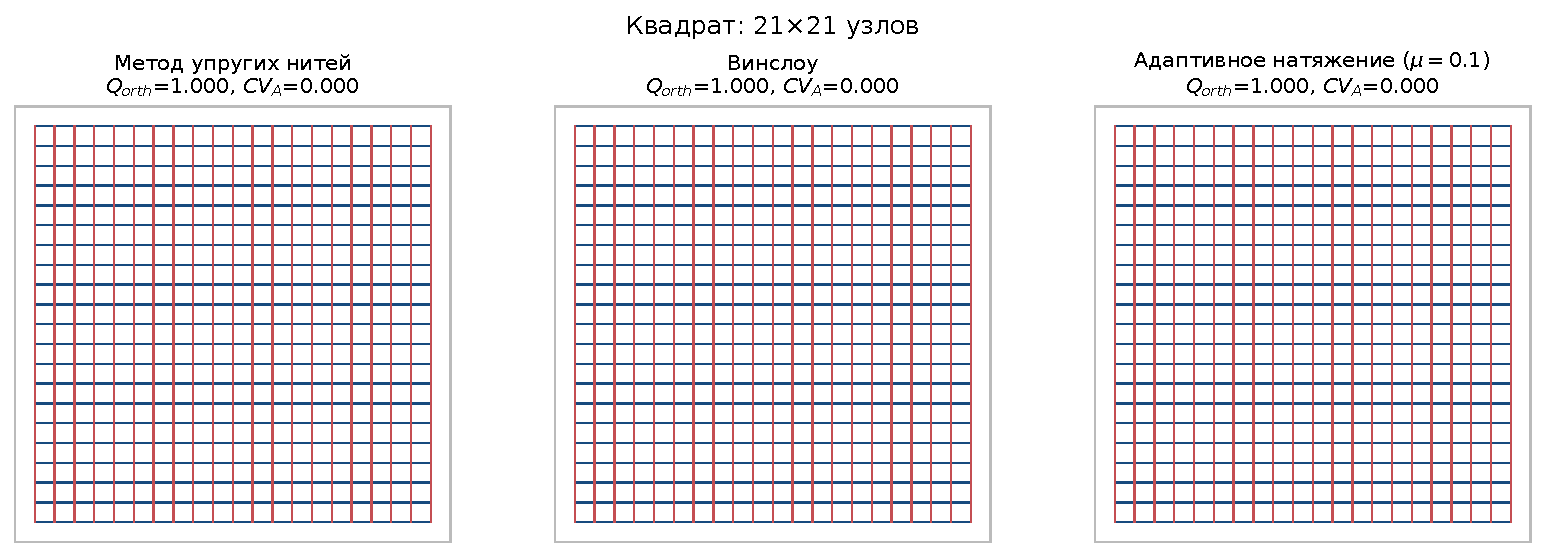
\includegraphics[width=\textwidth]{meshes_square.pdf}
\caption{Сетки квадрата. Все три функционала сохраняют точное аффинное
отображение.}
\label{fig:square}
\end{figure}

\begin{figure}[H]
\centering
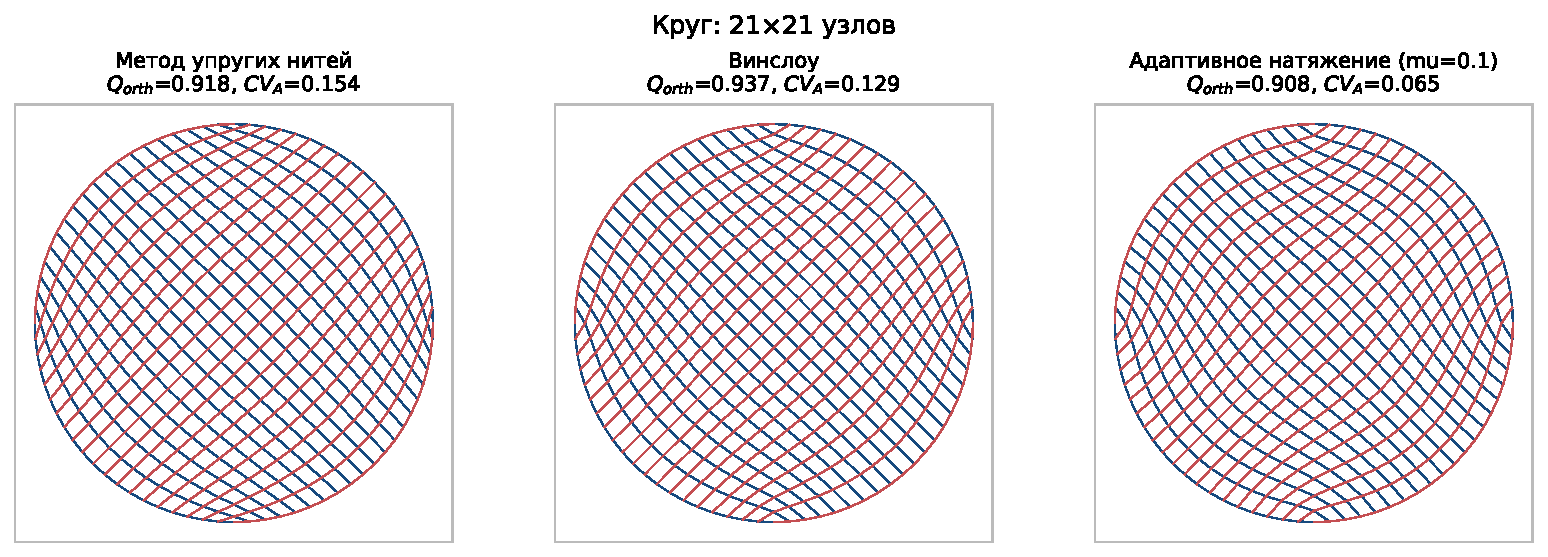
\includegraphics[width=\textwidth]{meshes_circle.pdf}
\caption{Сетки круга. Синие и красные линии соответствуют двум семействам
вычислительных координат.}
\label{fig:circle}
\end{figure}

\begin{figure}[H]
\centering
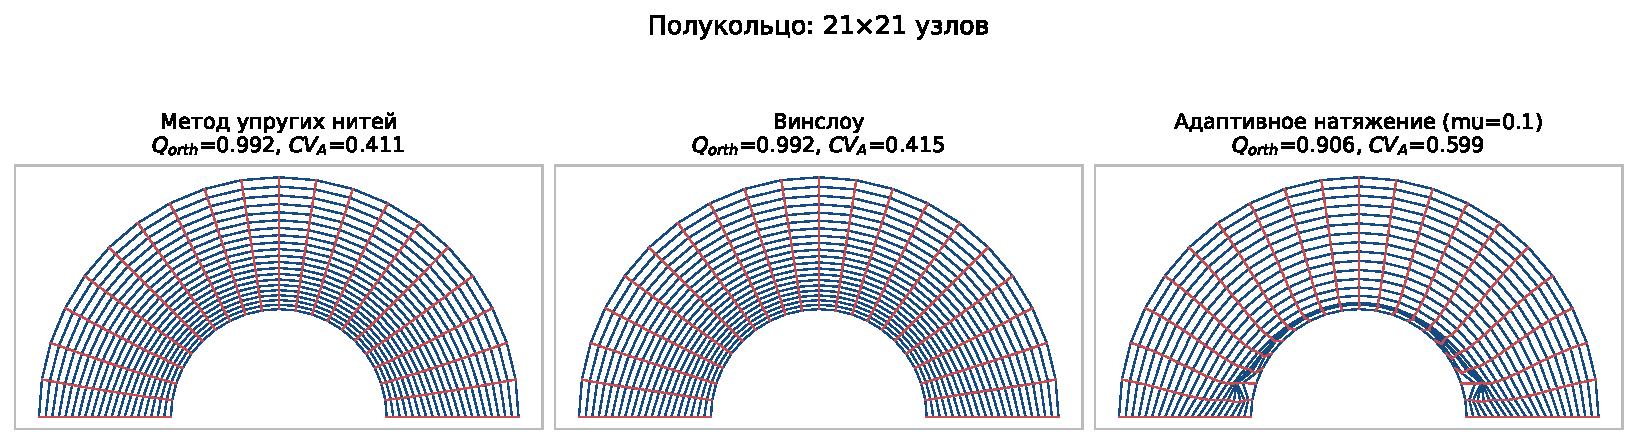
\includegraphics[width=\textwidth]{meshes_arch.pdf}
\caption{Сетки полукольца. Метод упругих нитей показан после
теоретически предусмотренной балансировки жёсткостей.}
\label{fig:arch}
\end{figure}

\begin{figure}[H]
\centering
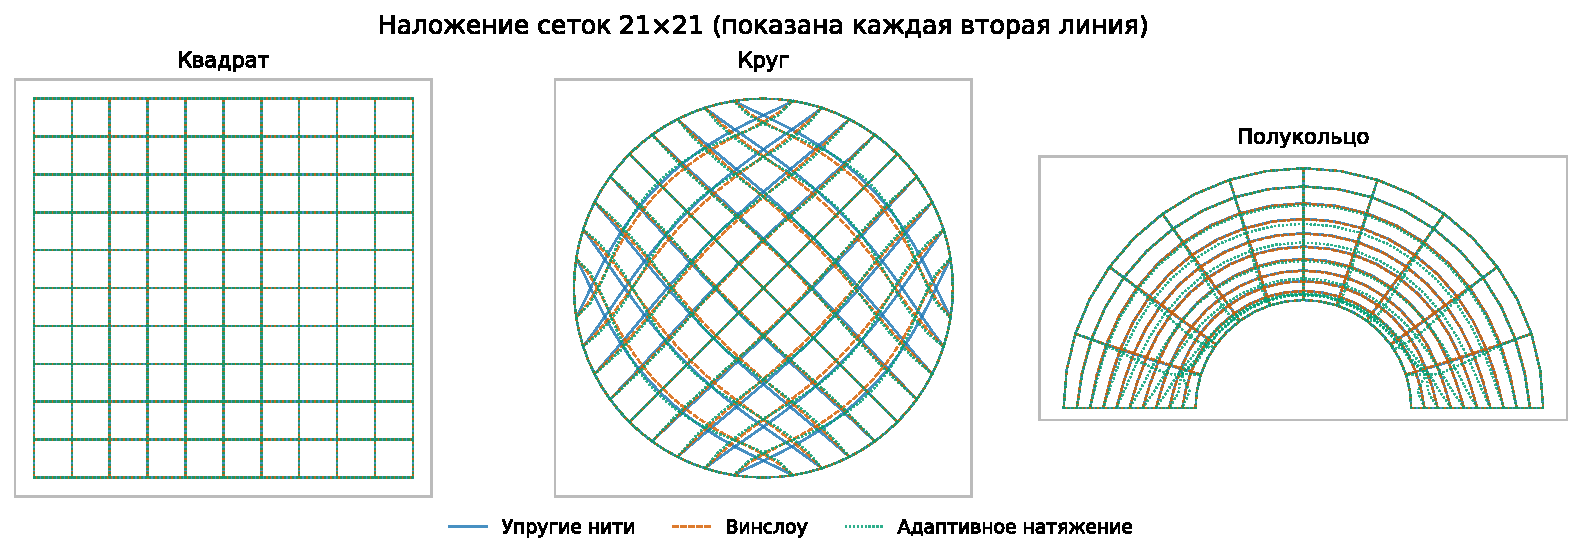
\includegraphics[width=\textwidth]{mesh_overlays.pdf}
\caption{Наложение сеток трёх методов. Для различимости показана каждая
вторая линия: метод упругих нитей --- сплошные синие линии, Винслоу ---
штриховые оранжевые, адаптивное натяжение --- точечные зелёные.
Совпадение в квадрате является аффинным контрольным случаем; расхождения
в круге и особенно в полукольце отражают различие функционалов.}
\label{fig:overlays}
\end{figure}

\FloatBarrier
\section{Обсуждение результатов}

Квадрат служит проверкой реализации: все методы дают
\(Q_{\mathrm{orth}}=1\), \(\Jsc=1\), \(N_{\mathrm{inv}}=0\),
\(CV_A\) на уровне ошибки округления и \(AR_{95}=1\). Нелинейным
методам не требуется ни одной итерации, поскольку сетка Кунса уже
стационарна.

В круге все три полученные дискретные сетки имеют положительные угловые
якобианы. Метод Винслоу имеет наибольшее
\(Q_{\mathrm{orth}}=0.9368\) против \(0.9183\) у метода упругих нитей
и \(0.9083\) у адаптивного натяжения. Адаптивное натяжение даёт
наименьший разброс площадей \(CV_A=0.0650\) и минимальный
\(AR_{95}=2.0006\). Во всех трёх полученных сетках одинаковое
\(\Jsc=0.0785\) достигается в фиксированных граничных углах
параметрического четырёхугольника на гладкой окружности. Перемещение
внутренних узлов может уменьшить этот глобальный минимум, но не
позволяет превысить заданную границей верхнюю оценку
\(\Jsc\le\sin(\pi/[2(N_\xi-1)])\). В отмеченных гладких ``углах'' диска
касательные соседних дуг совпадают, поэтому при сгущении границы эта
оценка стремится к нулю. Строгое условие
\eqref{eq:positive-j} здесь относится к внутренности; граничное
вырождение не позволяет сравнивать \(\Jsc\) круга между разными
разрешениями без этой оговорки.

Для полукольца балансировка первого метода сошлась к
\(k_\xi/k_\eta=0.06173208546\). Полученная сетка допустима и почти
совпадает по показателям с сеткой Винслоу:
\(Q_{\mathrm{orth}}=0.9922\), \(\Jsc=0.9569\) и \(0.9552\)
соответственно. Это принципиально меняет вывод по сравнению с
равножёстким вариантом: при \(k_\xi=k_\eta\) линейная система также
решается до машинной точности, но содержит 104 инвертированные ячейки и
имеет \(\Jsc=-0.99997\). Следовательно, проблема была не в самом первом
методе как таковом: в данном эксперименте причиной служила
невыполненная часть его теоретической настройки.

Регуляризованный функционал адаптивного натяжения при \(\mu=0.1\) в
полукольце сохраняет ориентацию, но даёт \(\Jsc=0.0290\),
\(CV_A=0.5989\) и \(AR_{95}=62.74\). Значит, положительный якобиан ещё
не обеспечивает хорошую форму ячеек. Контрольный запуск нормированного
варианта без логарифмического барьера (\(\mu=0\)) за 5000 итераций не
достиг критерия по градиенту и
приблизился к почти вырожденной сетке
\(\Jsc\approx1.2\cdot10^{-10}\). Поэтому опубликованные числа относятся
только к регуляризованной задаче при \(\mu=0.1\); влияние \(\mu\)
требует отдельного исследования и не позволяет приписывать результат
одной лишь исходной формуле~\eqref{eq:adaptive-original}.

Рис.~\ref{fig:overlays} делает различия видимыми непосредственно, а
табл.~\ref{tab:pairwise} сводит наиболее существенные попарные
изменения. Относительное изменение вычислялось по отношению к методу,
указанному после слова ``против''; знак улучшения зависит от показателя:
для \(Q_{\mathrm{orth}}\) и \(\Jsc\) лучше больше, для \(CV_A\) и
\(AR_{95}\) --- меньше.

\begin{table}[H]
\centering
\caption{Явное попарное сравнение результатов}
\label{tab:pairwise}
\small
\renewcommand{\arraystretch}{1.13}
\begin{tabular}{
  >{\raggedright\arraybackslash}p{22mm}
  >{\raggedright\arraybackslash}p{44mm}
  >{\raggedright\arraybackslash}p{85mm}}
\toprule
Область & Сравниваемые методы & Наблюдаемое различие \\
\midrule
Квадрат & Все три метода &
Сетки и все основные показатели совпадают с точностью округления. \\
Круг & Винслоу против упругих нитей &
\(Q_{\mathrm{orth}}\) выше на \(2.01\,\%\)
(\(0.9368\) против \(0.9183\)). \\
Круг & Адаптивный против Винслоу &
\(CV_A\) ниже на \(49.69\,\%\), \(AR_{95}\) ниже на \(2.24\,\%\),
но \(Q_{\mathrm{orth}}\) меньше на \(0.0285\). \\
Круг & Адаптивный против упругих нитей &
\(CV_A\) ниже на \(57.85\,\%\), \(AR_{95}\) ниже на \(18.60\,\%\),
но \(Q_{\mathrm{orth}}\) меньше на \(0.0100\). \\
Полукольцо & Упругие нити против Винслоу &
\(\Jsc\) выше на \(0.18\,\%\); остальные основные показатели
различаются менее чем на \(1.5\,\%\). \\
Полукольцо & Адаптивный против упругих нитей &
\(\Jsc\) ниже в \(33.00\) раза, \(AR_{95}\) выше в \(14.18\) раза,
\(CV_A\) выше на \(45.80\,\%\). \\
\bottomrule
\end{tabular}
\end{table}

Время в табл.~\ref{tab:results} приведено для одного запуска и
характеризует порядок затрат, а не строгий тест производительности.
Первый метод требует повторных линейных решений при балансировке;
нелинейные методы используют разные целевые функционалы. Число итераций
и невязки записаны в JSON для конкретного запуска и не являются сами по
себе сопоставимой мерой точности разных задач.

\section{Верификация и воспроизводимость}

Автоматический запуск содержит \AuditTestCount{} тестов. Проверяются
согласованность границ, сохранение граничных узлов, диспетчеризация
интерфейса, аффинные отображения, аналитические градиенты, остановка
оптимизатора и масштабная инвариантность. Добавлены независимые контроли:
точный объём скрученного куба на нескольких разрешениях, совпадение
двух- и пятиточечной тензорных квадратур, инвариантность суммарного
ориентированного объёма при перемещении внутренних узлов, форма ячеек
при различных числах узлов по направлениям и пример с положительными
угловыми, но отрицательным неугловым якобианом.

Дополнительная проверка градиентов использует сетки $5\times6\times7$
скрученного куба и $6^3$ шара с фиксированным возмущением, seed=22092026.
Для каждого функционала проверяются 24 координаты центральными
разностями с шагом $10^{-6}$; для адаптивного варианта взяты
$\mu\in\{0,0.01,0.1,1\}$. Нормированное расхождение определяется как
$|g_{\rm FD}-g|/\max(1,|g_{\rm FD}|,|g|)$.
Максимум в этом запуске равен $\AuditGradientError$; ошибки округления
и усечения из него не вычитаются. Это проверка выбранных точек, а не
доказательство градиента для всех входных данных.
Подробные условия, индексы координат, версии среды и результаты тестов
сохраняются в \texttt{output/audit/verification.json}.

Для полного численного воспроизведения из корня проекта:
\begin{quote}\ttfamily\scriptsize
python -m pip install -r requirements.txt\\
python audit\_reproduce.py --full\\
xelatex -interaction=nonstopmode -halt-on-error -output-directory=output/pdf article.tex\\
xelatex -interaction=nonstopmode -halt-on-error -output-directory=output/pdf article.tex\\
python build\_supplementary.py\\
python verify\_artifacts.py
\end{quote}
Для повторяемости затрат следует установить
\texttt{OPENBLAS\_NUM\_THREADS=1}; также задаётся \texttt{OMP\_NUM\_THREADS=1}.
Числа обсуждения 3D формируются из того же CSV, что и таблица.
Координаты всех 12 трёхмерных сеток сохранены отдельно, что позволяет
проверить метрики без повторной оптимизации. Архив сохраняет структуру
корня репозитория и содержит манифест SHA-256.
Сборка и интерактивное тестирование Windows-приложения являются
отдельной процедурой; успешные численные тесты в Linux не доказывают
работоспособность нового Windows EXE.

\FloatBarrier
\section{Трёхмерное обобщение}

Ниже сравниваются три трёхмерных алгоритма на одних и тех же
гексаэдральных областях. Второй алгоритм использует известную энергию
inverse mean ratio, а не функционал обратных гармонических координат.
Различие обозначений существенно: одинаковый исторический идентификатор
\texttt{winslow} в API не делает эти плотности математически тождественными.

\subsection{Гексаэдральная область и трансфинитная интерполяция}

Пусть \(\widehat\Omega=[0,1]^3\) --- вычислительный куб, а область
\(\Omega\subset\R^3\) задана шестью согласованными четырёхугольными
гранями \(\mathcal F_k^\pm\), по две в каждом координатном направлении.
Каждая грань --- поверхность, определённая двумя оставшимися
параметрами; её дискретное представление --- регулярный тензорный
набор точек с билинейной интерполяцией. Совместность граней по общим
рёбрам проверяется автоматически до начала расчётов.

Начальное отображение строится трансфинитной интерполяцией --- булевой
суммой трёх одномерных проекторов~\cite{thompson1985,coons1967}:
\begin{equation}
\vect r=\mathcal P_\xi\vect r+\mathcal P_\eta\vect r+\mathcal P_\zeta\vect r
-\mathcal P_\xi\mathcal P_\eta\vect r
-\mathcal P_\eta\mathcal P_\zeta\vect r
-\mathcal P_\zeta\mathcal P_\xi\vect r
+\mathcal P_\xi\mathcal P_\eta\mathcal P_\zeta\vect r,
\label{eq:tfi3d}
\end{equation}
где, например,
\(\mathcal P_\xi\vect r=(1-\xi)\vect r(0,\eta,\zeta)+\xi\vect r(1,\eta,\zeta)\).
Проектор \(\mathcal P_\xi\mathcal P_\eta\mathcal P_\zeta\) определяет
восемь вершин гексаэдра. Формула~\eqref{eq:tfi3d} воспроизводит шесть
граней точно; в автоматических тестах отклонение от граней шара не
превышает \(10^{-12}\).

\subsection{Функционалы}

В трёхмерной области метод упругих нитей представляет собой линейную
дискретную гармоническую задачу с весами
\(k_\xi,k_\eta,k_\zeta\), а балансировка обобщается на выравнивание
трёх суммарных энергий семейств нитей: условие
\(k_\xi S_\xi=k_\eta S_\eta=k_\zeta S_\zeta\) даёт
\(k_\eta/k_\xi=S_\xi/S_\eta\) и \(k_\zeta/k_\xi=S_\xi/S_\zeta\), что при
\(d=2\) совпадает с исправленной пропорцией
\(k_\xi/k_\eta=S_\eta/S_\xi\) из разд.~2.

Из обратных гармонических координат следует
$\int_{\widehat\Omega}\|\operatorname{cof}A\|_F^2/J$,
см.~\eqref{eq:winslow-3d}. В эксперименте минимизируется другая,
известная плотность inverse mean ratio~\cite{knupp2001}:
\begin{equation}
 I_{\rm MR}=\int_{\widehat\Omega}\frac{\|A\|_F^2}{J^{2/3}}\,d\xi\,d\eta\,d\zeta,
 \qquad A=(\vect r_\xi,\vect r_\eta,\vect r_\zeta),\quad J=\det A>0.
 \label{eq:winslow3d}
\end{equation}
В размерностно-индексированном семействе
$\int_{[0,1]^d}\|A_d\|_F^2/(\det A_d)^{2/d}\,d\boldsymbol\xi$
при $d=2$ получается двумерная плотность Винслоу; при $d=3$ это
\eqref{eq:winslow3d}, но не $\|\operatorname{cof}A\|_F^2/J$.
Нельзя получать двумерный случай ограничением трёхмерной карты на
плоскость: тогда трёхмерный определитель обращается в нуль.
Куб даёт постоянную плотность 3 и нулевой внутренний градиент.
Дискретная энергия равна среднему восьми угловых плотностей по каждой
ячейке, умноженному на её вычислительную меру. Ограничение на угловой
якобиан сохраняет допустимость именно этих отсчётов, не всей ячейки.
При изотропном схлопывании плотность формы остаётся постоянной, поэтому
отдельный нижний порог якобиана необходим и не заменяется энергией формы.

Функционал адаптивного натяжения обобщается через нормированный
метрический тензор
\(\widetilde D=G/J_*^{2/3}\), где \(G\) --- метрический тензор
отображения (\(g_{11}=|\vect r_\xi|^2\),
\(g_{12}=\vect r_\xi\cdot\vect r_\eta\), и т.\,д.),
а $J_*>0$ --- фиксированный ориентированный объём численной аппроксимации
границы на опорной сетке с $\max(N_\xi,N_\eta,N_\zeta,21)$ узлами
по каждому направлению, а не точный объём аналитического шара:
\begin{equation}
I_{\rm A}=\int_{\widehat\Omega}
\left[
\frac{(\tr\widetilde D-3)^2}{\det\widetilde D}
+(\det\widetilde D-1)^2
\right]d\xi\,d\eta\,d\zeta
-\mu\int_{\widehat\Omega}\ln\frac{J}{J_*}\,d\xi\,d\eta\,d\zeta.
\label{eq:adaptive3d}
\end{equation}
Здесь \(\tr\widetilde D=(g_{11}+g_{22}+g_{33})/J_*^{2/3}\) и
\(\det\widetilde D=(J/J_*)^2\). Тождественное отображение куба даёт
\(\tr\widetilde D=3\), \(\det\widetilde D=1\) и нулевую плотность; при
\(d=2\) формула переходит в двумерную~\eqref{eq:adaptive-original} с
нормировкой \(\widetilde D=D/J_*\). Оба
нелинейных функционала минимизируются по внутренним узлам
методом L-BFGS с аналитическим градиентом. Вычисления ведутся
в нормированных координатах $\vect r/J_*^{1/3}$; целевые нормы
бесконечности градиента равны $2\cdot10^{-6}$ для inverse mean ratio
и $2\cdot10^{-5}$ для адаптивного варианта. Эти разные допуски фиксируют
собственные критерии остановки, но не эквивалентную ошибку решений. Дискретизация использует
восемь односторонних троек производных каждой гексаэдральной ячейки;
градиент каждой тройки собирается цепным правилом по восьми углам.
Параметр $\mu$ умножает $-\ln(J/J_*)$, а не $-\ln\det\widetilde D$:
последняя запись изменила бы силу барьера вдвое.
Контроль градиентов описан в разделе верификации.

\subsection{Метрики качества и границы геометрической проверки}

Минимальный масштабированный якобиан $\Jsc$ по-прежнему берётся по
восьми углам каждой ячейки. Отдельно вычисляется минимум обычного
якобиана в 27 тензорных точках $\{0,1/2,1\}^3$ локального куба.
$N_{\mathrm{inv}}$ в таблице 3D обозначает число ячеек, в которых
хотя бы один из этих отсчётов неположителен; это диагностическое,
а не полное число всех возможных инверсий. Положительность 27 отсчётов
не гарантирует положительности между ними и не доказывает глобальную
взаимную однозначность сетки. Для полной проверки необходим иной
алгоритм оценки полинома якобиана, например подход с коэффициентами
Бернштейна~\cite{johnen2017}; в этой версии он не реализован.
Флаг сходимости требует выполнения критерия оптимизатора и положительности
диагностических отсчётов. Контроль 27 точек выполняется после решения,
тогда как барьер внутри оптимизатора относится к восьми углам.

Коэффициент ортогональности усредняется по трём парам направлений на
внутренних узлах. $AR_{95}$ --- 95-й процентиль отношения наибольшего
и наименьшего сингулярных чисел \emph{локальной} матрицы ячейки в её центре.
Это не показатель только угла $(0,0,0)$ и не обусловленность карты всего
вычислительного куба. На декартовой сетке с различным шагом по направлениям
он равен отношению наибольшего и наименьшего размера ячейки, а не обязательно 1.

Для трилинейной ячейки определитель локальной матрицы Якоби является
полиномом степени не выше двух по каждой переменной. Поэтому её
ориентированный объём точно в точной арифметике вычисляется тензорной
квадратурой Гаусса $2\times2\times2$:
\[
 V_c=\frac18\sum_{a,b,c\in\{-,+\}}\det B(t_a,t_b,t_c),
 \qquad t_\pm=\frac12\pm\frac{1}{2\sqrt3}.
\]
Среднее восьми \emph{угловых} якобианов в общем случае не является этим
интегралом. $CV_V$ вычисляется по полученным объёмам ячеек.
Точность квадратуры относится к кусочно-трилинейной сетке, а не к
точному объёму лежащей за ней аналитической криволинейной области.

\subsection{Вычислительный эксперимент}

Рассмотрены четыре области: куб \([-1,1]^3\) (аффинный контроль),
скрученный куб (верхняя грань повёрнута на \(0.6\) рад относительно
нижней; точный объём \((8/3)(2+\cos0.6)\)), шар из шести
гномонических сферических граней и арковая призма --- сечение
полукольца разд.~5, выдавленное вдоль вертикальной оси. Основная серия
использует \(11^3\) узлов; для шара предел \(9^3\) объясняется в
конце раздела. Результаты сведены в табл.~\ref{tab:results3d} и на
рис.~\ref{fig:3d-twisted}--\ref{fig:3d-overlays}.

\begin{table}[H]
\centering
\caption{Показатели трёхмерных сеток (для шара --- \(9^3\) узлов,
для остальных областей --- \(11^3\))}
\label{tab:results3d}
\scriptsize
\resizebox{\textwidth}{!}{\begin{tabular}{llrrrrrrr}
\toprule
Область & Метод & $Q_{\rm orth}$ & $\sigma_{\rm len}$ & $J_{\min}^{\rm sc}$ & $N_{\rm inv}$ & $CV_V$ & $AR_{95}$ & $t$, мс \\
\midrule
Куб & Метод упругих нитей (3D) & 1.0000 & 2.34e-16 & 1.0000 & 0 & 1.26e-15 & 1.0000 & 20.6514 \\
Куб & Винслоу (3D) & 1.0000 & 3.59e-16 & 1.0000 & 0 & 2.07e-15 & 1.0000 & 21.0997 \\
Куб & Адаптивное натяжение (3D, mu=0.1) & 1.0000 & 3.59e-16 & 1.0000 & 0 & 2.07e-15 & 1.0000 & 19.0569 \\
Скрученный куб & Метод упругих нитей (3D) & 0.9854 & 0.0078 & 0.9227 & 0 & 0.0269 & 1.4259 & 514.7244 \\
Скрученный куб & Винслоу (3D) & 0.9856 & 0.0081 & 0.9227 & 0 & 0.0239 & 1.4278 & 89.9571 \\
Скрученный куб & Адаптивное натяжение (3D, mu=0.1) & 0.9856 & 0.0090 & 0.9227 & 0 & 0.0096 & 1.4397 & 88.1820 \\
Шар & Метод упругих нитей (3D) & 0.9847 & 0.0176 & 0.0722 & 0 & 0.4184 & 4.0579 & 9.2401 \\
Шар & Винслоу (3D) & 0.9897 & 0.0262 & 0.0722 & 0 & 0.3667 & 2.7522 & 98.7227 \\
Шар & Адаптивное натяжение (3D, mu=0.1) & 0.9689 & 0.0457 & 0.0722 & 0 & 0.2193 & 3.9170 & 169.0627 \\
Арковая призма & Метод упругих нитей (3D) & 0.9990 & 0.1146 & 0.9513 & 0 & 0.3651 & 5.1704 & 609.3075 \\
Арковая призма & Винслоу (3D) & 0.9996 & 0.1154 & 0.9662 & 0 & 0.3190 & 5.1427 & 287.2753 \\
Арковая призма & Адаптивное натяжение (3D, mu=0.1) & 0.9933 & 0.1143 & 0.8112 & 0 & 0.4083 & 8.6554 & 310.5916 \\
\bottomrule
\end{tabular}
}
\end{table}

\begin{figure}[htbp]
\centering
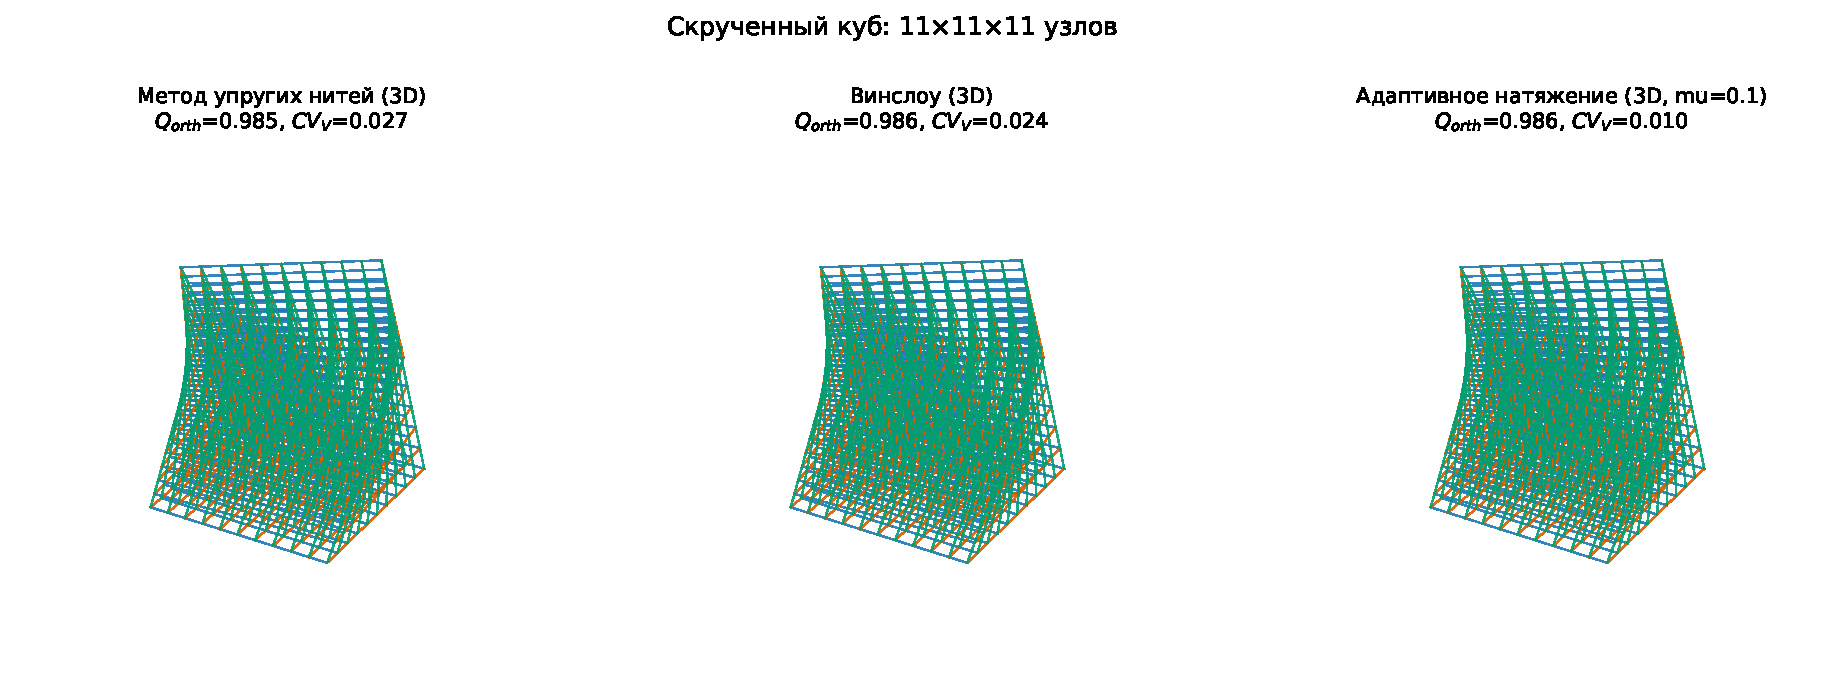
\includegraphics[width=0.92\textwidth]{meshes3d_twisted.pdf}
\caption{Сетки скрученного куба \(11^3\). Синим, оранжевым и зелёным
показаны три семейства вычислительных координат.}
\label{fig:3d-twisted}
\end{figure}

\begin{figure}[htbp]
\centering
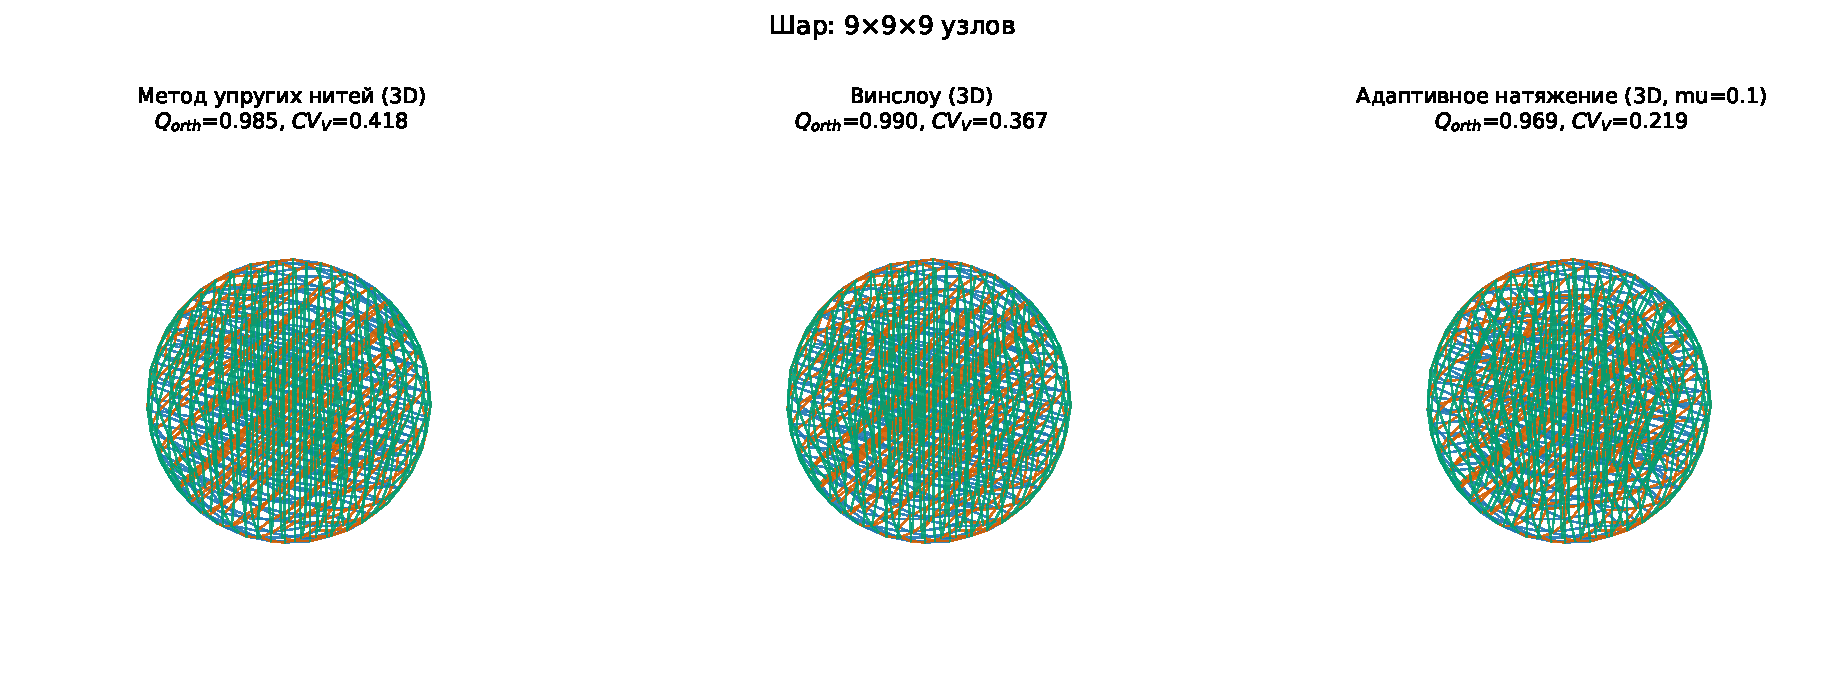
\includegraphics[width=0.92\textwidth]{meshes3d_ball.pdf}
\caption{Сетки шара \(9^3\) на шести гномонических гранях.}
\label{fig:3d-ball}
\end{figure}

\begin{figure}[htbp]
\centering
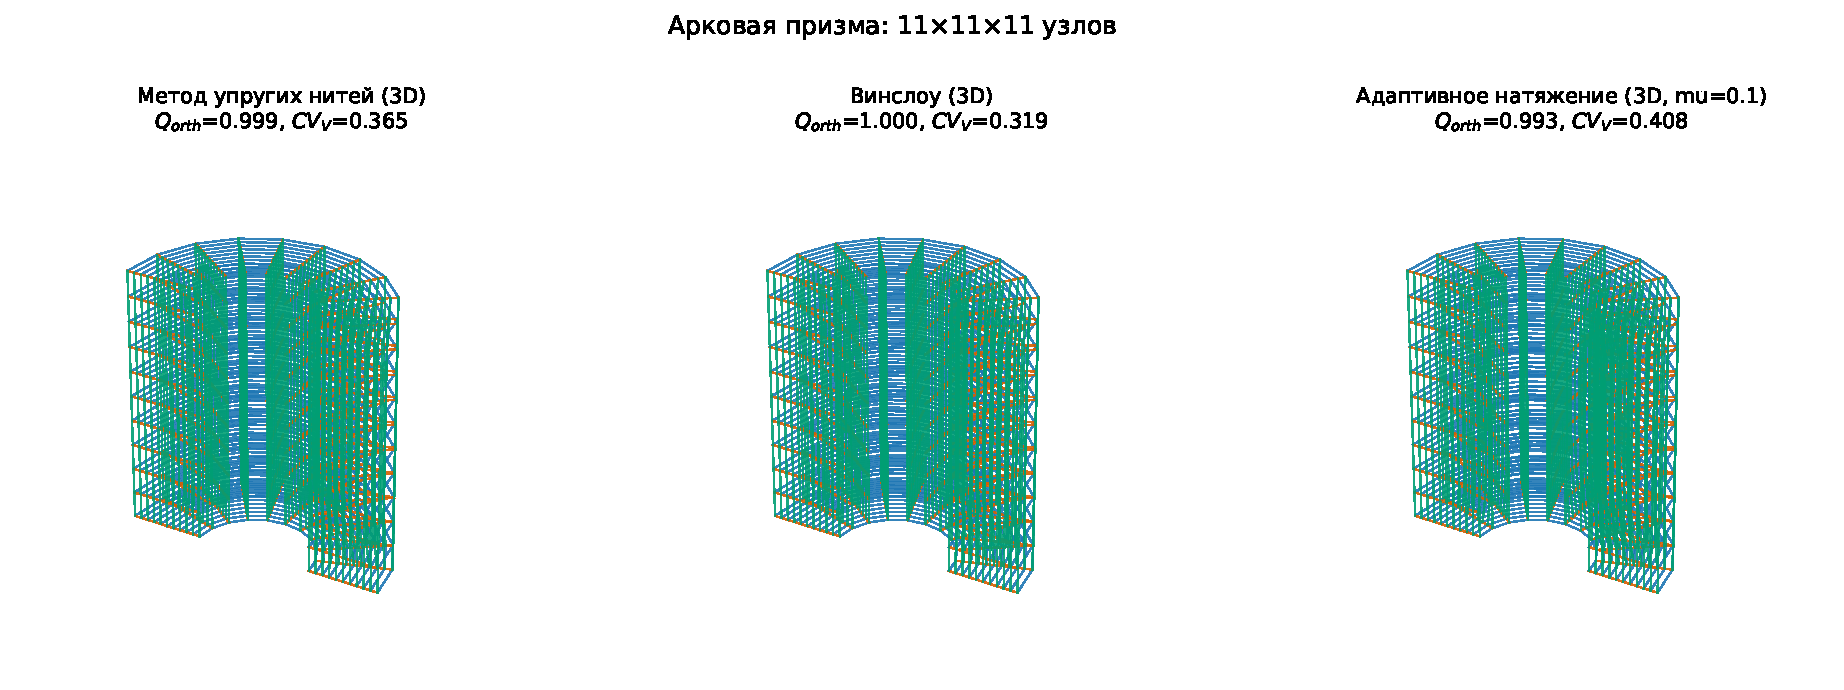
\includegraphics[width=0.92\textwidth]{meshes3d_arch_prism.pdf}
\caption{Сетки арковой призмы \(11^3\): упругие нити после
балансировки, inverse mean ratio и адаптивное натяжение.}
\label{fig:3d-prism}
\end{figure}

\begin{figure}[htbp]
\centering
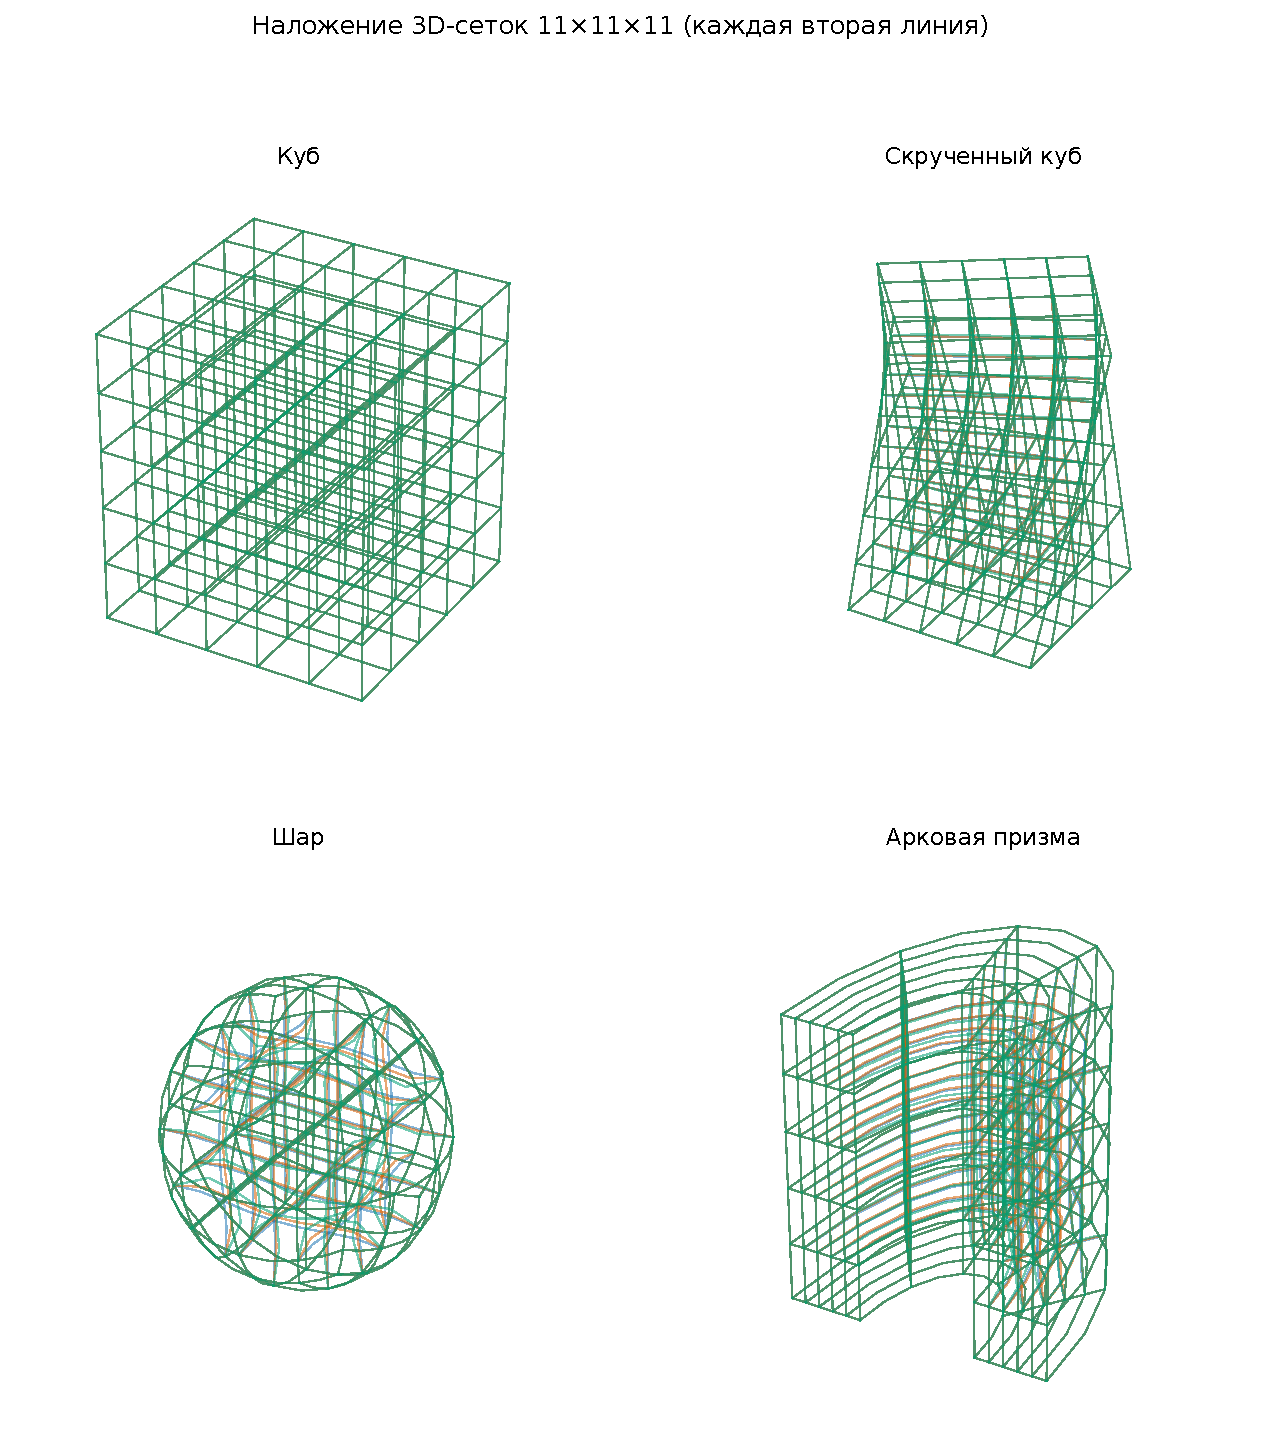
\includegraphics[width=\textwidth]{mesh_overlays_3d.pdf}
\caption{Наложение трёхмерных сеток (каждая вторая линия).
Синий --- упругие нити, оранжевый --- inverse mean ratio, зелёный --- адаптивное
натяжение. В кубе линии совпадают; в остальных областях различия
видны как смещение семейств.}
\label{fig:3d-overlays}
\end{figure}

Для призмы балансировка даёт $k_\eta/k_\xi\approx16.8$, близкое к
двумерному значению 16.2. Близость не является тождеством: суммы
включают разное число граничных и внутренних рёбер. Отдельный контроль
равножёсткого варианта и его сравнение со сбалансированным сохранены
в \texttt{output/audit/verification.json}.

% Generated by audit_reproduce.py from results_3d.csv; do not hand-edit numbers.
В скрученном кубе адаптивный вариант при $\mu=0.1$ даёт
$CV_V=0.0096$ против $0.0239$ у inverse mean ratio
(снижение на $59.7\,\%$). Значения ортогональности близки, но не тождественны:
$0.985550$ и $0.985561$ соответственно.
В шаре inverse mean ratio имеет наибольший среди трёх методов
$Q_{\rm orth}=0.9897$ и наименьший
$AR_{95}=2.1021$; адаптивный вариант даёт меньший разброс
объёмов: $CV_V=0.2212$ против $0.3684$,
но уступает по ортогональности.

В арковой призме inverse mean ratio имеет наибольший $Q_{\rm orth}$ и
наибольшее значение минимального углового масштабированного якобиана, а также наименьшие $CV_V$ и $AR_{95}$
в проверенной тройке. Его $AR_{95}=4.9563$, тогда как для
адаптивного варианта $AR_{95}=8.2422$.
Однако по размерному показателю $\sigma_{\rm len}$ адаптивный вариант лучше:
$0.1143$ против $0.1154$.
Поэтому превосходство по \emph{всем} метрикам не утверждается.
Это наблюдения при указанных разрешениях, границе, начальной сетке и параметрах,
а не универсальный рейтинг функционалов и не оценка ошибки решения уравнения.


Шар выявил типичное для гладких областей ограничение. В углах
параметрического гексаэдра, лежащих на гладкой границе, касательные
трёх координатных линий компланарны, поэтому угловой якобиан
\(J\to0\) при сгущении сетки, а его знак в билинейной
дискретизации может измениться: уже при \(11^3\) узлов начальная сетка
Кунса гномонического шара содержит отрицательные угловые якобианы.
Поэтому шар используется с разрешением \(9^3\), а в интерактивной программе для этого пресета
максимальное число узлов ограничено девятью. Величина
\(\Jsc=0.0722\) у всех трёх методов достигается в фиксированных углах
границы и соответствует двумерному эффекту разд.~7: глобальный минимум
масштабированного якобиана задаётся границей, а не выбором функционала.

Сравнение использует одинаковые граничные узлы и разрешение внутри
каждой области; нелинейные методы начинают с одной TFI-сетки. Балансировка
упругих нитей является отдельным алгоритмическим этапом и входит в его
время. Основное $\mu=0.1$ не подбиралось для равного качества всех областей;
выводы нельзя переносить на другие $\mu$ без исследования чувствительности.
Проверка градиентов при нескольких $\mu$ не является таким исследованием
качества сеток. Времена единичных запусков не служат строгим бенчмарком.

\FloatBarrier
\section{Программная реализация и интерактивный интерфейс}

\subsection{Архитектура приложения}

На общем вычислительном ядре создано настольное приложение для
интерактивного построения и исследования структурированных сеток.
Программа разделена на три уровня. Модуль \texttt{mesh\_methods.py}
содержит геометрию, три решателя и метрики; он не зависит от
интерфейса. Модуль \texttt{mesh\_gui\_model.py} хранит редактируемую
границу, проверяет параметры, сериализует проект и непосредственно
диспетчеризует выбранный метод. Tk-контроллер
\texttt{mesh\_gui.py} отвечает только за элементы управления,
визуализацию Matplotlib, события мыши и фоновый запуск расчёта. Такое
разделение позволяет тестировать геометрическое редактирование и выбор
решателя без создания окон.

Выбор метода в интерфейсе однозначно вызывает соответствующую функцию
ядра. Для упругих нитей используется флаг балансировки жёсткостей; поля
числа итераций, допуска и \(\mu\) не участвуют в линейном решении. Для
Винслоу используются максимум итераций и допуск по норме градиента, а
для адаптивного натяжения дополнительно применяется \(\mu\). Неактивные
для выбранного метода поля сохраняются видимыми, но пояснение под ними
явно указывает, какие значения войдут в текущий расчёт. Допустимы
\(5\le N_\xi,N_\eta\le81\), от 1 до \(10^5\) итераций, положительный
допуск и \(\mu\ge0\).

\subsection{Трёхмерный режим}

Приложение имеет переключатель размерности и переключатель языка
интерфейса (русский/английский), действующий на все надписи, метрики и
сообщения. В трёхмерном режиме доступны
четыре области --- куб, скрученный куб, шар и арковая призма --- и те же
три метода с общими решателями ядра. Число узлов задаётся независимо по
трём направлениям в диапазоне от 5 до 21; для шара верхняя граница
ограничена девятью из-за вырождения угловых ячеек гномонической
параметризации. Вращение сцены выполняется левой кнопкой мыши, масштаб
--- правой кнопкой или колесом; кнопки ракурсов («изометрия», «сверху»,
«спереди», «сбоку»)
и поворота задают готовые виды, а линии трёх направлений \(\xi,\eta,\zeta\)
окрашиваются в разные цвета с легендой в углу сцены; нити сортируются по
глубине с затуханием дальних линий, поэтому сетка читается без
визуального «каше», а внешняя оболочка области выделяется светлой рамкой
поверх сетки, так что боковые грани остаются видны при любом ракурсе.
Рамка координатных
осей скрыта. Редактирование границы в трёхмерном режиме не
предусмотрено. Показатели качества соответствуют разделу о трёхмерном
обобщении: \(Q_{\mathrm{orth}}\), \(\Jsc\), число инвертированных ячеек,
\(CV_V\), объём области и \(AR_{95}\). CSV-экспорт в трёхмерном режиме
записывает кортежи \(i,j,k,x,y,z\). Формат проекта дополнен полем
размерности: для 3D сохраняются выбранная область и численные параметры,
для 2D --- редактируемая граница как ранее; файлы формата версии 1
обоих типов открываются без изменений.

\subsection{Задание области и интерактивное редактирование}

Граница представляется четырьмя ориентированными против часовой стрелки
полилиниями в порядке ``низ, правая сторона, верх, левая сторона''.
Общие углы соседних сторон хранятся согласованно: перенос угла
одновременно изменяет обе примыкающие полилинии. Пользователь может
начать с квадрата, круга или полукольца, выбрать независимые
\(N_\xi\) и \(N_\eta\), пересэмплировать текущую границу либо получить
пользовательскую область одним из пяти режимов:
перемещением углов, отдельного узла границы, стороны целиком, всей
области или внутреннего узла готовой сетки. Активные объекты выбираются
левой кнопкой мыши по ближайшему маркеру на экране.

Во время изменения границы показывается быстрая трансфинитная сетка
Кунса; она визуально отделена от результата выбранного решателя. После
отпускания мыши проверяются согласованность углов, конечность координат,
положительная ориентация и отсутствие самопересечений полилинейной
границы. Недопустимая область выделяется цветом и не передаётся
решателю. По желанию пользователя допустимая граница автоматически
перестраивается после каждого перетаскивания; иначе расчёт запускается
отдельной кнопкой. Кнопки ``Сбросить'' и ``Вписать'' соответственно
возвращают эталонную геометрию и подбирают масштаб области просмотра.

Ручной перенос внутреннего узла выполняется только после построения
сетки и не запускает оптимизацию. Метрики немедленно пересчитываются,
однако флаг сходимости аннулируется и результат маркируется как ручная
правка. Тем самым геометрический эксперимент пользователя не
представляется как решение исходной вариационной задачи.

\subsection{Расчёт, диагностика и обмен данными}

Перед запуском ещё раз проверяются параметры и граница. Решатель
выполняется в отдельном рабочем потоке, а Tk-цикл с периодом 70 мс
проверяет очередь результата. Поэтому окно и индикатор выполнения не
зависают; изменяющие состояние элементы временно блокируются, чтобы
геометрия не могла измениться посреди расчёта. Исключение численного
метода перехватывается и выводится как диагностическое сообщение, не
завершая приложение.

Таблица результата содержит признак подтверждённой сходимости, число
итераций, время, линейную невязку или норму градиента,
\(Q_{\mathrm{orth}}\), \(\Jsc\), \(N_{\mathrm{inv}}\), \(CV_A\) и
\(AR_{95}\). При отсутствии подтверждённой сходимости сетка всё равно
показывается вместе с сообщением решателя и геометрическими метриками,
что позволяет отличить остановку оптимизатора от инверсии или плохой
формы ячеек.

Проект сохраняется в UTF-8-файл \texttt{*.mesh.json}: в него входят
версия формата, четыре полилинии, размеры сетки, выбранный метод, его
численные параметры и режим перетаскивания. Вычисленная сетка
намеренно не сериализуется и после открытия проекта строится заново.
Экспорт CSV записывает для каждого узла \(i,j,x,y\) с 17 значащими
цифрами координат, а экспорт PNG сохраняет текущее поле визуализации с
разрешением 220 dpi.

Самодостаточная сборка для 64-разрядной Windows имеет каталожный формат.
Исполняемый файл \texttt{MeshGridStudio.exe} расположен рядом с
подкаталогом \texttt{runtime}. При запуске библиотеки не распаковываются во
временный каталог, что сокращает время старта; установленный
интерпретатор Python не требуется. Интерфейс учитывает масштабирование
DPI Windows. Два встроенных режима проверки создают все виджеты и
решают тестовую задачу каждым из трёх методов уже внутри собранного
приложения.

\begin{figure}[H]
\centering
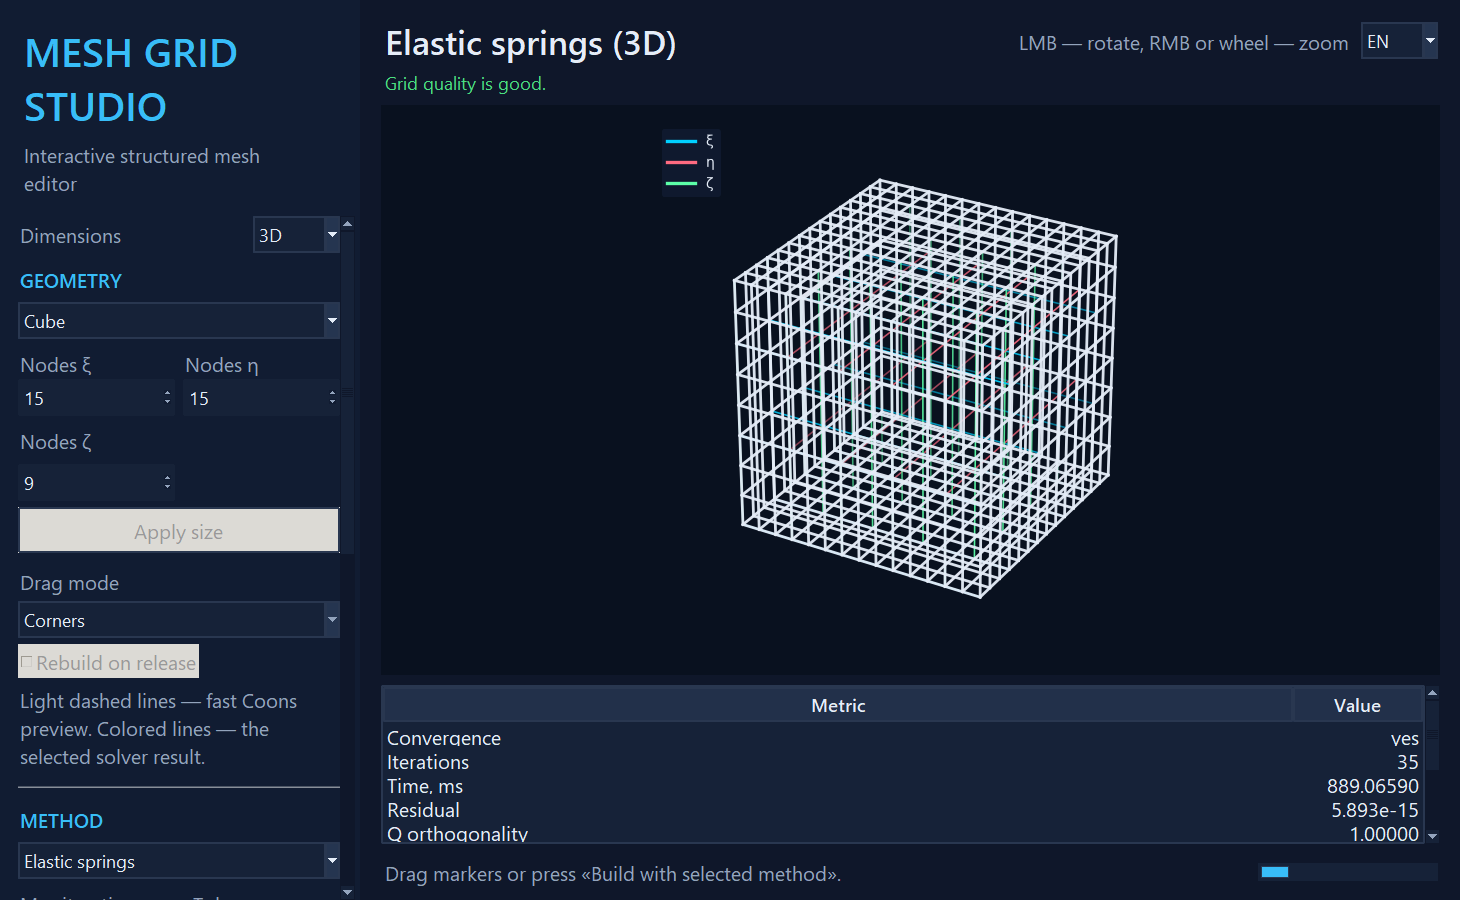
\includegraphics[width=0.94\textwidth]{docs/ui-preview.png}
\caption{Интерактивная программа: выбор метода, редактирование границы
и отображение показателей допустимости и качества сетки.}
\label{fig:gui}
\end{figure}

\begin{figure}[H]
\centering
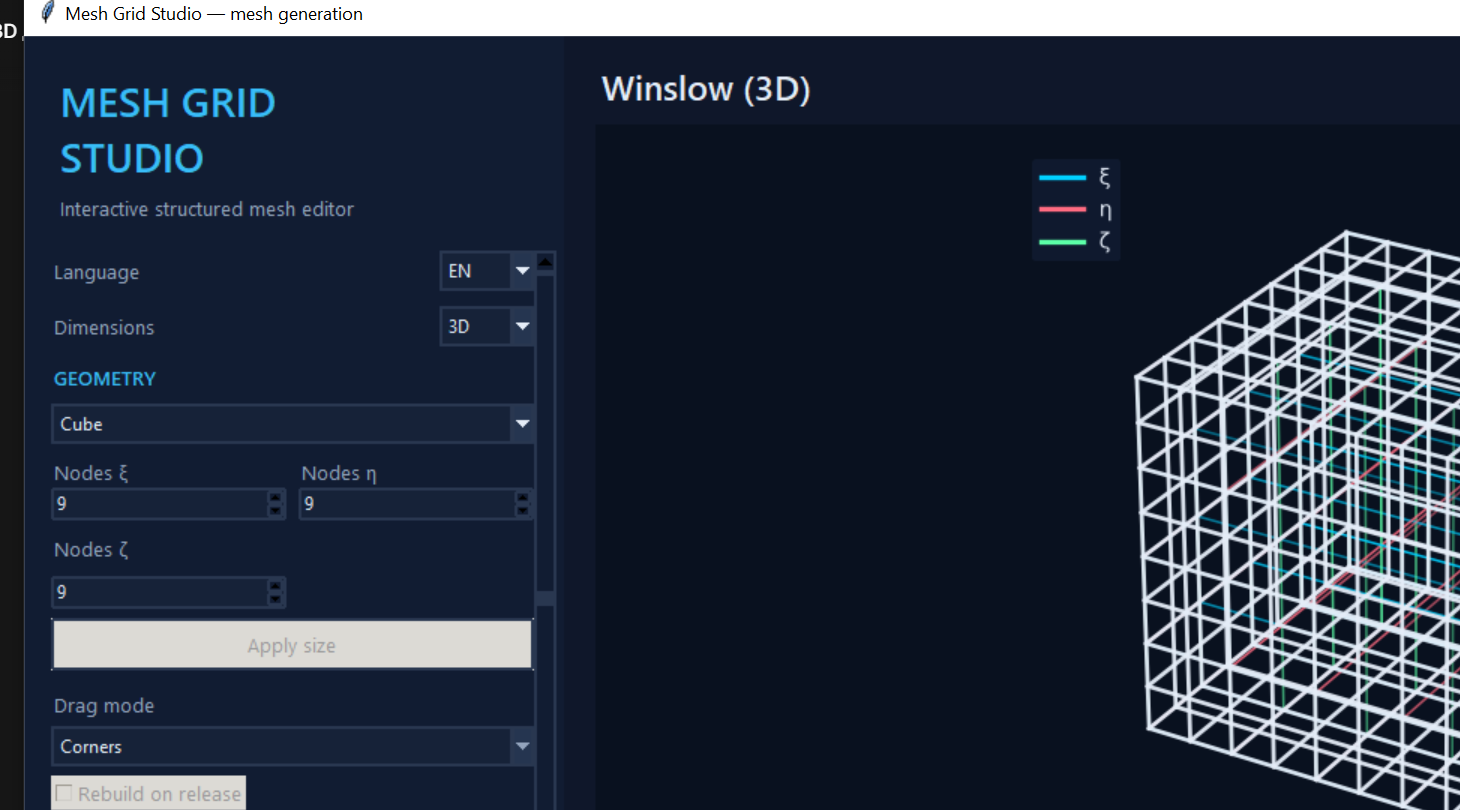
\includegraphics[width=0.94\textwidth]{docs/ui-preview-3d.png}
\caption{Иллюстрация интерфейса до научного аудита (прежнее название метода): цветовое различие направлений
\(\xi,\eta,\zeta\), подсветка граничной оболочки и панель ракурсов.}
\label{fig:gui3d}
\end{figure}

\FloatBarrier
\section{Заключение}

Получены три программные реализации, соответствующие выписанным
дискретным постановкам, в пространствах размерности два и три. Для
метода упругих нитей балансировка
жёсткостей в полукольце привела к
\(k_\xi/k_\eta=0.06173208546\) и устранила все 104 инвертированные
ячейки равножёсткого варианта; в трёхмерной арковой призме то же
правило сошлось к \(k_\eta/k_\xi=16.8\) и также устранило инверсии.
В круге наибольшую ортогональность
\(Q_{\mathrm{orth}}=0.9368\) обеспечил метод Винслоу, а
регуляризованное адаптивное натяжение дало наименьшие
\(CV_A=0.0650\) и \(AR_{95}=2.0006\).

В трёхмерном эксперименте известная энергия inverse mean ratio
сопоставлена с упругими нитями и нормированным метрическим функционалом.
Исправлены вычисление объёмов, трактовка локальной формы ячейки и объём
геометрической проверки. Численные сравнения приведены в табл.~\ref{tab:results3d}
и в обсуждении, сформированном из CSV. Сохранены различия критериев:
уменьшение разброса объёмов не обязательно сопровождается улучшением
ортогональности или формы ячеек. Научный приоритет известных плотностей
не заявляется; самостоятельная новизна сравнения требует дополнительного
сопоставления с профильной литературой и независимыми реализациями.

Единственного лучшего метода в рассмотренных задачах нет. Для круга
Винслоу предпочтителен, если приоритетна ортогональность; адаптивное
натяжение при \(\mu=0.1\) предпочтительно по равномерности площадей и
отношению сторон, но уступает по ортогональности. Для полукольца
сбалансированный метод упругих нитей и Винслоу дают практически
совпадающие допустимые сетки, причём первый имеет немного лучшие
\(\Jsc\), \(CV_A\) и \(AR_{95}\). Адаптивное натяжение с тем же
\(\mu\) для этой области неприемлемо по форме ячеек. Таким образом,
метод следует выбирать по целевой характеристике сетки и геометрии
области, а не по одному названию функционала или факту сходимости
оптимизатора.

Эксперимент также выявил ограничение метрического функционала. Его
нормированный вариант без логарифмического барьера при \(\mu=0\) не
достиг критерия сходимости за 5000 итераций, тогда как барьерная
регуляризация при \(\mu=0.1\) сохранила ориентацию, но в полукольце
дала \(AR_{95}=62.74\). Поэтому малой
невязки или одного положительного якобиана недостаточно: верификация
должна одновременно включать проверку аналитического градиента,
ориентации и независимых характеристик формы и размера ячеек.
Нормированные расхождения градиента не превосходят
$\AuditGradientError$ в описанном дополнительном контроле, а
\AuditTestCount{} автоматических тестов прошли в зафиксированной среде.
Эти результаты подтверждают проверенные свойства реализации, но не
полноту всех возможных сценариев, новизну метода или допустимость
каждого гексаэдра между диагностическими точками.

Исследование ограничено сетками \(21\times21\) и \(9^3\)--\(11^3\),
тремя двумерными и четырьмя трёхмерными областями, одним
начальным приближением Кунса, фиксированными граничными узлами и
основным значением \(\mu=0.1\). Не проводились исследование сходимости
по шагу сетки, строгий тест быстродействия и решение модельного
дифференциального уравнения; поэтому геометрические показатели нельзя
интерпретировать как оценку ошибки последующего численного решения.
Приложение даёт воспроизводимый интерактивный доступ к трём решателям
и метрикам качества в двух и трёх измерениях.

\begingroup
\footnotesize
\raggedright
\begin{thebibliography}{99}
\setlength{\itemsep}{0.1em}
\setlength{\parsep}{0pt}

\bibitem{samarskii1989}
Самарский А.\,А.
\textit{Теория разностных схем}.
М.: Наука, 1989.

\bibitem{godunov1967}
Годунов С.\,К., Прокопов Г.\,П.
О расчётах конформных отображений и построении разностных сеток.
\textit{ЖВМ и МФ}. 1967. Т.~7, №~5. С.~1031--1059.

\bibitem{winslow1966}
Winslow A.\,M.
Numerical solution of the quasilinear Poisson equation in a nonuniform
triangle mesh.
\textit{Journal of Computational Physics}. 1966. Vol.~1, no.~2.
P.~149--172.

\bibitem{tikhonov1999}
Тихонов А.\,Н., Самарский А.\,А.
\textit{Уравнения математической физики}.
М., 1999.

\bibitem{ivanenko1988}
Иваненко С.\,А., Чарахчьян А.\,А.
Криволинейные сетки из выпуклых четырёхугольников.
\textit{Журнал вычислительной математики и математической физики}.
1988. Т.~28, №~4. С.~503--514.

\bibitem{thompson1985}
Thompson J.\,F., Warsi Z.\,U.\,A., Mastin C.\,W.
\textit{Numerical Grid Generation: Foundations and Applications}.
Amsterdam: North-Holland, 1985.

\bibitem{coons1967}
Coons S.\,A.
\textit{Surfaces for Computer-Aided Design of Space Forms}.
Technical Report MAC-TR-41. 1967.

\bibitem{liu1989}
Liu D.\,C., Nocedal J.
On the limited memory BFGS method for large scale optimization.
\textit{Mathematical Programming}. 1989. Vol.~45. P.~503--528.
doi: 10.1007/BF01589116.

\bibitem{armijo1966}
Armijo L.
Minimization of functions having Lipschitz continuous first partial
derivatives.
\textit{Pacific Journal of Mathematics}. 1966. Vol.~16, no.~1.
P.~1--3. doi: 10.2140/pjm.1966.16.1.

\bibitem{knupp2001}
Knupp P.\,M. Algebraic Mesh Quality Metrics.
\textit{SIAM Journal on Scientific Computing}. 2001. Vol.~23, no.~1.
P.~193--218. doi: 10.1137/S1064827500371499.

\bibitem{huang2015}
Huang W., Kamenski L., Russell R.\,D.
A comparative numerical study of meshing functionals for variational mesh adaptation.
\textit{Journal of Mathematical Study}. 2015. Vol.~48, no.~2. P.~168--186.
doi: 10.4208/jms.v48n2.15.04. arXiv:1503.04709.

\bibitem{johnen2017}
Johnen A., Weill J.-C., Remacle J.-F.
Robust and efficient validation of the linear hexahedral element.
2017. arXiv:1706.01613v3.

\bibitem{tishkin2024}
Тишкин В.\,Ф.
\textit{Описание программы построения расчётной сетки}.
Неопубликованная рукопись, полученная автором в порядке личного
сообщения. Б.\,м., б.\,г.

\bibitem{khalilov2024}
Халилов Д.\,Э.
\textit{Сравнение различных вариационных принципов построения расчётных
сеток}.
Выпускная квалификационная работа бакалавра. М., 2024.

\end{thebibliography}
\endgroup

\end{document}
